\input{settings}

\begin{comment}

to find all files that contain a term (useful for creating index)

grep -r term * | grep tex | sed 's/:/ /g' | awk '{print $1}' | sort | uniq

\end{comment}

\newcommand{\progpath}{\basepath/programs}

\makeatletter
\def\seealso#1#2{{\em see also\/} #1, #2}
\makeatother


\begin{document}

\begin{comment}
reduce space

titlesec
http://www.ctex.org/documents/packages/layout/titlesec.pdf
wrapfig

\end{comment}

% \frontmatter
\title{Software Engineering for Machine Learning }
\author{Yung-Hsiang Lu
and George K. Thiruvathukal}
\maketitle

   
     

   

\tableofcontents
\listoffigures
\listoftables


\newcommand{\frontpath}{\basepath/frontmatter}
\chapter*{Foreword}



\begin{flushright}
{\it } 

\end{flushright}


 

\newpage
\chapter*{Preface}

\section*{Why Is This Book Needed?}

There are hundreds of books about software engineering, softwawre
development, programming, software testing ...  There are also many
books on artificial intelligence, machine learning, and related
topics. Many books and movies decribe future worlds where machines are
capable of learning, reasoning, and making decisions.
Why do we write this book?  Why should you spend time reading
this book?  How is this book different from any other book?  Like many
authors, we want to write this book because we perceive a need for it.
{\it Because we think there is a need for this book.}


\begin{tabular}{|p{4in}|}
  {\it The problem is that there are too many books on these topics.
    These books are independent of each other.  Instead, this book
    resides at the intersection of three topics: software engineering,
    machine learning, and programming.  }
\end{tabular}  

Few Software Engineering books show programs. Some Machine Learning
books show programs that implementing algorithms but never explain how
to manage the software.  Very few programming books talk about
applications of machine learning.  As these fields become increasingly
important and deeply intertwined, a book that integrates these topics
becomes essential.  This is that book.

Why is it necessary to have a book that covers all three topics
simultaneously?  Existing university education is strucuted into
majors: accounting, biology, computer science, electrical engineering,
literature, mathematics, statistics, theatre, and so on.  Each major
has a curriculum and students take sequences of courses building their
expertise in the particular field. Each course focuses on a specific
topic.  It is expected that a student would become an expert in the
field after taking a series of courses.  This approach, however, often
lead to the situations where people ``can see trees but overlook
forests'' because they cannot ``connect the dots''.  This is
understandable because each course focuses on depth (i.e., ``trees'')
and without teaching how to see forests.  This traditional approach is
no longer valid becasue rapid technology progresses make integration
necessary.  {\it Multidisciplinary} projects are everywhere.

Is there a need for a book, any book, on any subject since almost
everything is now available on the Internet?  Any book becomes
obsolete at the moment when it is published.  The difference between
books and the Internet is that books (good books) can provide
systematic approaches to learning. The Internet is excellent looking
up answers for specific questions. However, in many cases, asking the
right questions requires deep understanding of the topics.  This
creates a circular problem: Without deep understanding, it is
difficult to ask meaningful questions and find useful answers. Without
useful answers, it is difficult to learn and acquire deep
understanding to ask the right questions.

\section*{Principles in Writing this Book}

This book is different from most (maybe all) available books.
We set a few principles when writing this book:

\begin{itemize}
\item This book emphasizes actions. Readers are asked to {\it do
  things} because doing is the best way to learn.

\item This book eliminates as much redudant materials as
  possible.  There is no history about machine learning
  of software engineering; there are already many books
  on these subjects.

\item This book is written for ``advanced beginners'': they have
  already written some programs solving small (``toy'')
  problems. Also, this book does not explain how to manage your
  computer.  There are already hundreds of books about
  how to use computers and install software packages.

\item This book is not a dictionary nor an encyclopedia.
  It is intended to provide readers with actionable
  knowledge so that they can learn enough basic skills
  and look up additional information on the Internet.

\item This book provides good ways to solve common problems.
  The book does not intend to explain all possible ways
  solving all possible problems. Many useful solutions

\item This book uses free tools. Everything mentioned in
  this book is free of charge.

\item This book solves ``real'' problems.  Most books
  use simplified problems 
  
\end{itemize}  




\newpage
\chapter*{Author, Reviewers, and Artist}

\section*{Author}

\index{ACM|see{Association for Computing Machinery}}
\index{Association for Computing Machinery} Yung-Hsiang Lu is a
professor at the School of Electrical and Computer Engineering in
Purdue University, West Lafayette, Indiana, U.S.A.  He is an ACM
(Association for Computing Machinery) Distinguished Scientist and ACM
Distinguished Speaker. He published ``Intermediate C Programming''
(CRC Press, ISBN 9781498711630).  This book provides deep insight
about how to prevent, detect, and remove software defects (i.e.,
``bugs'').  Dr. Lu and three Purdue students founded a Perceive
Inc. This technology company uses video analytics to improve shopping
experience in stores. This company receives two Small Business
Innovation Research (SBIR-1 and SBIR-2) grants from the National
Science Foundation.  Dr. Lu received the Ph.D. degree from the
Department of Electrical Engineering in Stanford University,
California, U.S.A.  \\

George K. Thiruvathukal is a Professor of Computer Science at Loyola
University Chicago.  He has published two books about software
engineering.


\section*{Artist}


The book's cover is painted by Kyong Jo Yoon.  Yoon is a Korean artist
and often places heroic figures in natural settings.  He is an adviser
of the Korean Fine Arts Association and his work is on display in the
Ann Nathan Gallery in Chicago, Illinois, U.S.A.







% \input{frontmatter/rules}


\mainmatter

\begin{comment}
Part1: Software Tools and Development Process
   Chapter 0: Python Basics
   Chapter 1: Version Control, Pull Requests
   Chapter 2: Continuous Integration, Unit Tests
   Chapter 3: Branch and Web Services
   Chapter 4: Documentation
   Chapter 5: Graphics Packages
\end{comment}

\renewcommand{\thispartpath}{\basepath/software}

\part{Software Engineering}

\renewcommand{\thischapterpath}{\thispartpath/python}
\chapter{Introduction to Python}

\def\tightlist{}

In this chapter~\footnote{This chapter is adapted from Thiruvathukal, Christopher, and Shafaee, \emph{Web Programming in Python}, 2002. Rights have been reverted to the authors for this out-of-print work. It is also being updated for Python 3, which is what we use exclusively in this book.}, we will
examine the basic facilities of the Python programming language, and go
on to the more advanced features in the next.

\subsection{Characteristics of Python}
\label{characteristics-of-python}

Here is a high-level look at the
features of Python, for those with a background in programming
languages.

\paragraph{Scripting} 
Python is a scripting language.
This loosely means that you do not have to compile Python programs;
Python can execute them directly. In fact, you can type lines directly
into the Python interpreter and have it execute them interactively.
Python does compile programs into code it interprets, but it will handle
the compilation itself, without troubling you.

\paragraph{Nondeclarative}
Python programs consist of
executable statements. They don't have declarations. In most languages,
you declare a function; in Python, you execute a statement that creates
a function object and assigns it to a variable. In other languages, you
call a function by giving its name and an argument list. The Python call
looks exactly the same, but instead of the name of the function, you
specify the name of the variable containing the function as its value.

\paragraph{Typeless or dynamically typed language} That means that variables do not have
static (declared)types; values have types. Variables are not declared. A value of any
type may be assigned to any variable.

\paragraph{High-Level}
Python is a high-level language. It
has high-level data structures built into the language, such as
dictionaries that allow you to associate values with objects. As of
Python2, Python has had a garbage collector. You allocate objects
whenever you need them, but you don't have to delete them. When there is
no way left for the program to access the object, when there are no
pointers left that point to it, Python automatically frees its storage.
Older versions of Python also deallocate objects automatically with a
reference count scheme, which will not reclaim storage of circularly
linked, inaccessible structures.

\paragraph{Modular}
Python programs are organized as
collections of modules kept in libraries. Each module is kept in a
separate file, and the libraries in directories. A good programming
practice, when writing larger programs, is to use as many preexisting
modules as possible and to divide the code you do write into
general-purpose modules. These modules can be debugged individually and
can be reused in other programs.

\paragraph{Object-Oriented}
Python has facilities that allow
object-oriented programming. It has classes and inheritance, as any
proper object-oriented programming language should. But Python is not
perfectly object oriented. Python does not provide private or otherwise
restricted scopes for names. The information-hiding aspects of
object-oriented programming are on the honor system.

\paragraph{With Operator Declarations}
Python allows you to create
functions for the built-in operators, to be used when the operators are
applied to instances of certain classes. This allows you to implement
abstract data types, new types of objects with their own set of
operators. The operators include subscripting operators, so you can
implement new types of objects that behave like arrays.

\paragraph{With Metaprogramming Facilities}
What Python calls metaprogramming,
other languages refer to as introspection or reflection. The program
itself can examine and modify its interpreter's own state and components
while it is running. This is useful for debugging and for changing the
running program under program control.

\subsection{Executing Programs}
\label{executing-programs}

\paragraph{Interactive Use}
\label{interactive-use}
You can execute Python from the
command line in a command window. It will come up with a greeting and a
command prompt (\verb">>>").~\footnote{Python is easy to run on Linux, OS X, and Windows. For Windows, we recommend installing Windows Subsystem for Linux to get a complete Linux shell environment. To be covered in preliminaries section.}

\begin{verbatim}
$ python
Python 3.6.5 (default, Apr  1 2018, 05:46:30) 
[GCC 7.3.0] on linux
Type "help", "copyright", "credits" or "license" for more information.
>>> 
\end{verbatim}

You type Python statements at the
command prompt, and Python executes them immediately. If you type an
expression, Python will evaluate it and type out the value.

\begin{verbatim}
>>> 12+14+20
46
\end{verbatim}

We will use the command interpreter
to try out Python features to show how they work.

Python statements can extend beyond
the end of a line, in which case the interpreter will give a different
prompt (\verb"...") for the continuation:

\begin{verbatim}
>>> (1+2
...   )*3
9
\end{verbatim}

Python can't always figure out
that you wish to continue a statement to another line. The way you force
it to continue to the next line is to put a backslash, \textbackslash{},
as the last character on a line. This is customary in Unix-like systems.
It incorporates the following character, the newline, into the current
line as white space.

\paragraph{Scripts in Files}

You can also place programs in
files and execute them from there. For example, you can edit a file
SayHi in the current directory, containing:

\resetlinenumber[1]
\linenumbers
\begin{tt}
  \lstinputlisting{\thischapterpath/hello/SayHi.py}
\end{tt}
\nolinenumbers

Then set SayHi's execute permissions and execute it:

\begin{verbatim}
chmod a+x SayHi.py
\end{verbatim}

\begin{verbatim}
$ ./SayHi.py
Hello
\end{verbatim}

You can also run the script \emph{explicitly} with Python:

\begin{verbatim}
$ python3 SayHi.py
Hello
\end{verbatim}

is a comment to the shell, the command interpreter on Linux. It tells the
shell that the way to execute this file is to execute the program in
file \texttt{/usr/bin/python} , and pass it the rest of the file as its
input. The print statement tells Python to write out the string Hello on
the standard output, which will write it to you. The \emph{print} is
required when Python is executing a script in a file. When you are
typing directly to it, Python knows to write out the values of
expressions, but when it is executing scripts, it assumes you do not
want the value of every expression you execute cluttering up your
output, so it will not write out the values of expressions.

\subsection{Arithmetic Expressions}

\paragraph{Arithmetic Types}

Python has four built-in arithmetic data types:

\begin{enumerate}
\item fixed sized (at least 32-bit) signed integers
\item variably sized, unbounded precision signed integers
\item floating point approximations to real numbers
\item complex numbers (with real and imaginary parts) for engineering calculations. We will not consider complex numbers further, since they are not typically relevant to Web enterprise applications.
\end{enumerate}

Integer literals can be written in
decimal, octal, or hexadecimal (base 16) format using the same syntax as
in C or C++:

\begin{itemize}

\item
  Octal integers begin with 0 and
  contain only octal digits (0-7). Strangely, that means zero is written
  in octal.
\item
  Decimal integers begin with a
  decimal digit other than zero and contain only decimal digits.
\item
  Hexadecimal integers begin with
  0x or 0X. The prefix is followed by a string of hexadecimal digits,
  0-9, a-f, A-F. The letters A, B, . . . F, of course, represent the
  values, 10, 11, . . . 15.
\end{itemize}


\begin{verbatim}
>>> 20
20
>>> 020
020
>>> 0x20
16
\end{verbatim}

Long integers are written as an
integer followed with an L (in uppercase or lowercase, but lowercase is too
hard to distinguish from the digit one). The difference between integer
and long integer is that integers are fixed sized. Integer arithmetic
will overflow if the results get too large. Long integers occupy as much
storage as they need. Long integer arithmetic does not overflow.~\footnote{GKT: Latest releases of Python 2 and 3 do not overflow. This needs to be revised.} For
example, 2 \emph{32} cannot be represented in 32 bits. So here is what
happens when we try to take two to the 32nd power, written \emph{2**32}
in Python:


\begin{verbatim}
>>> 2**32
4294967296
\end{verbatim}


\begin{verbatim}
>>> 2L**32
4294967296L
\end{verbatim}

%(This example also shows Python's
%response to an error.)

Since integers occupy single
machine words, computers perform integer arithmetic very fast. Long
integer arithmetic typically requires much more time.

Floating point numbers are written
with a decimal point or an exponent, or both. For example: \texttt{.2},
\texttt{2.0}, \texttt{20.}, \texttt{2000e-1}, \texttt{2E3}.

Python allows mixed-mode
arithmetic, as we saw above with \texttt{2L**32} . If the two operands of
an arithmetic operator have different types, Python will convert them to
a common type. Python converts the operand whose type has the smaller
range of values to the type of the operand with the wider range of
values. (This is called a widening coercion: The ``narrower'' operand is
forced to be the type of the wider.) So, if they are mixed in
expressions, integers will be converted to long integers or floats, and
long integers will be converted to floats. The conversions to float may
lose some low-order digits.


Table 2-1 is a complete list of
Python operators and their precedence levels. Some of the operators
won't be discussed until later sections; we'll refer to the table then.
The operators with higher precedence levels are performed before those
with lower precedence.

The arithmetic operators in Python
are much the same as those in C or C++. They are at precedence levels 9
through 12. The bit-wise operators (ANDs, ORs, shifts) are mostly at
levels 5 through 8. Since they are not used much in Web enterprise
applications, we won't discuss them further.

We will discuss the logical and
comparison operators later when we discuss \texttt{while} loops.

\begin{longtable}{l|p{3cm}|p{7cm}}
\toprule
Precedence & Operators & Comments \\
\midrule
  1 & \texttt{x or y} &  This is the logical OR operation.
It will return true if either \texttt{x} or \texttt{y} is true, i.e.
non-zero. Like the \texttt{\textbar{}\textbar{}} operator in C, it is
short-circuited: It will not evaluate \texttt{y} if \texttt{x} determines
the value of the expression. It first evaluates \texttt{x} and returns the
value of \texttt{x} if \texttt{x} is not zero. If \texttt{x} is zero, it
evaluates and returns the value of \texttt{y} . By ``x is zero'' we mean
that it would be considered zero in an \texttt{if} or \texttt{while}
expression. Other values than a number zero also count as zero. \\
%
\midrule
  2 & \texttt{x and y} & This is the logical AND operation.
It will return true if both \texttt{x} and \texttt{y} are true, i.e.
non-zero. Like the \texttt{\&\&} operator in C, it is short-circuited: It
will not evaluate \texttt{y} if \texttt{x} determines the value of the
expression. It first evaluates x and returns \texttt{x} if \texttt{x} is
zero. If \texttt{x} is not zero, it evaluates and returns the value of
\texttt{y} . By ``x is zero'' we mean that it would be considered zero in
an \texttt{if} or \texttt{while} expression. Other values than a number zero
also count as zero. \\
%
\midrule
  3 & \texttt{not x} & This is the logical NOT operator. 
It returns 1 if \texttt{x} is zero; it returns 0 if \texttt{x} is anything
else. \\
%
\midrule
  4 & \verb"x < y", \verb"x > y", \verb"x <= y", and \verb"x >= y"  & The relational operators are much
like they are in other languages. Operators \verb"!=" and \verb"<>" both mean not equal. \\
%
   & \verb"x == y", \verb"x != y", \verb"x <> y"  & Testing for equality, \verb"==" and \verb"!=", can be applied to structured objects as discussed later.
They attempt to find out if the structured objects have equal
components. \\
%
   & \verb"x is y", \verb"x is not y", \verb"x in y", \verb"x not in y"  & Operators \verb"x is y" and \verb"x is not y"
test whether two names reference the same object, so they will be much
faster than \verb"==" and \verb"!=" for structured objects, but they don't perform the
same test.  We will discuss \verb"x in y" and \verb"x not in y" later, when we discuss sequence types.\\
%
\midrule
  5 & \verb"x | y" &  This is the bitwise OR operation,
ORing the corresponding bits in two integers. \\
%
\midrule
  6  & \verb"x ^ y" & This is the bitwise EXCLUSIVE-OR (XOR) operation, XORing the corresponding bits in two integers. \\
%
\midrule

  7 & \verb"x & y" & This is the bitwise AND operation,
ANDing the corresponding bits in two integers. \\
%
\midrule

8 & \verb"x << y", \verb"x >> y" & These are the shift operators.
They apply to integers or long integers. The bits in \texttt{x} are
shifted left ( \texttt{\textless{}\textless{}} ) or right (
\texttt{\textgreater{}\textgreater{}} ) the number of positions indicated
by \texttt{y} . The right shifts are arithmetic: The sign bit will be
shifted in at the top, preserving the sign of the \texttt{x} operand. \\
%
\midrule
9 & \verb"x + y", \verb"x - y" & Addition and subtraction. Operator
\texttt{+} also performs concatenation on sequences, as we will see later.\\
%
\midrule
10 & \verb"x * y", \verb"x / y", \verb"x % y" & Multiplication, division, and
modulus (or remainder). Operator \texttt{\%} will also work with floating
point numbers. Operator \texttt{*} also applies to sequence types, and
operator \texttt{\%} has a special function for strings. We will look at
these other uses later.\\
%
\midrule
11 & -y, ~y, +y & Negation, bitwise complement, and
unary plus (no operation for numbers).\\
%
\midrule
12 & \verb"x ** y" & Exponentiation, $x^y$ \\
%
\midrule
13 & \verb"f(...)" & Function call \\
%
 & \verb"x.attr" & attribute access \\
%
 & \verb"x[i]" & subscripting \\
%
 & \verb"x[i:j]" & slicing \\
%
\midrule
14 & \verb"(...)" & construct tuple \\
%
 & \verb"[...]" & construct list \\
%
 & \verb"{...}" & construct dictionary \\
%
 & \verb"`...`" & construct string \\
%
\bottomrule
\end{longtable}


\subsection{Built-in Arithmetic Functions}
\label{built-in-arithmetic-functions}

Python has a number of built-in functions you can call.
Other mathematical functions can be found in module \texttt{math}.
Complex arithmetic functions are in module \texttt{cmath}.


\begin{longtable}{l|p{7cm}}
\toprule
Function call & Explanation \\
%
\midrule
\verb"v = abs(x)" & the absolute value of \texttt{x} \\
%
\midrule
\verb"v = cmp(x, y)" & Compares \texttt{x} and \texttt{y} and
assigns \texttt{v} a negative value if \texttt{x\textless{}y} , zero if
\texttt{x==y} , and positive if \texttt{x\textgreater{}y} \\
%
\midrule
\verb"u,v = coerce(x, y)" & Determines the common type for
\texttt{x} and \texttt{y} required for arithmetic operators then assigns
\texttt{x} converted to that type to \texttt{u} and \texttt{y} converted to
that type to \texttt{v} \\
%
\midrule
\verb"u,v = divmod(x,y)" & are integers or long integers, it assigns \texttt{u=x/y} and \texttt{v=x\%y} .
If \texttt{x} and \texttt{y} are floating point numbers, it assigns
, the largest integer less than or equal to \texttt{x/y,} and \\
%
\midrule
\verb"v=float(x)" & the value of \texttt{x} converted to a floating point value \\
%
\midrule
\verb"v=int(x)" & the value of \texttt{x} converted to an integer value \\
%
\midrule
\verb"v=long(x)" & the value of \texttt{x} converted to a long integer value \\
%
\midrule
\verb"v=complex(x)" and \verb"v=complex(x,y)" & Converts \texttt{x} to a complex
number, or \texttt{x} to the real part and \texttt{y} to the imaginary part of a complex number \\
%
\midrule
\verb"v=max(x1, x2, ...)"  &  Assigns \texttt{v}  with the largest value of x1, x2, ... \\
%
\midrule
\verb"v=min(x1, x2, ...)"  &  Assigns \texttt{v}  with the smallest value of x1, x2, ... \\
%
\midrule
\verb"v=pow(x,y)"  & Assigns v the value of \texttt{x} raised to the \texttt{y} power, \texttt{x**y} \\
%
\midrule
\verb"v=pow(x, y, z)" & Assigns v  the value of \texttt{x} raised to the \texttt{y} power modulus \texttt{z} , i.e., \texttt{x**y\%z} \\
%
\midrule
\verb"v=round(x)" &  Assigns v the the floating point number \texttt{x} rounded to have \texttt{n} digits after the decimal
point. If you omit \texttt{y}, it defaults to zero. \\
%
\bottomrule
\end{longtable}

\subsection{Assignments and Variables}
\label{assignments-and-variables}

Variables are not declared. You create a variable simply by assigning a value to it. The simplest form of an assignment is:

\begin{verbatim}
variable = expression
\end{verbatim

For example

\begin{verbatim}
>>> a=10
>>> a
10
>>> b=a+2
>>> b
12
\end{verbatim}

Variable names and other identifiers in Python are composed of letters, digits, and underscore
characters. The first character of the identifier must not be a digit.  The letters are the ISO-Latin characters A-Z and a-z.
\footnote{Python also provides full UNICODE support.}

You can also do several assignments on the same line; for example let's swap the values of \emph{a} and
\emph{b} :


\begin{verbatim}
>>> a,b
(10, 12)
>>> a,b = b,a
>>> a,b
(12, 10)
\end{verbatim}

We will look at this again later.
Note also that we can list more than one expression on a line in
interactive mode and Python will write out all their values. Both the
multiple assignments and the multiple values on a line use tuples, a
kind of sequence which we will discuss in
\href{chap2.html\#92836}{Tuples}.

\subsection{Creating Functions}
\label{creating-functions}

You may create a function and assign it to a variable with the \emph{def} statement, for example:


\begin{verbatim}
>>> def diff(x,y):
...    return abs(x-y)
...
>>> diff(-10.5)
15
\end{verbatim}


creates a function \texttt{diff} that returns the absolute difference between values \emph{x} and \emph{y}.
There are several things to note about this function creation:

\begin{enumerate}

\item
  The \texttt{def} line introduces
  the code for the function. It gives the name we will call the
  function, \emph{diff} , and the argument list. The function will be
  called with two arguments, \emph{x} and \emph{y} . The \emph{def} line
  is terminated with a colon.
\item
  The name \texttt{diff} is not
  exactly the name of the function. It is a variable that is assigned
  the function as a value. It is an assignment as much as assigning
  \emph{diff=value} would be, and indeed, \emph{diff} can be reassigned.
\item
  The body of the function is
  indented. All statements in the same group of statements must be
  indented the same amount. Soon we'll look at \emph{while} statements,
  whose bodies must be indented beneath the \emph{while} .
\item
  The function returns a value with a \emph{return} statement.
\item
  If there is no \texttt{return} statement, the function does not return a value, and the call of the
  function should be used only as a statement, not within an expression.
\item
  A function is called by the form
  \emph{f(args)} where \emph{f} is a variable containing the function
  and \emph{args} are the arguments being passed in.
\end{enumerate}

When you use a variable name in a
function, Python will look in three places to try to find what it means:

\begin{enumerate}

\item
  The function's local variables.
  The arguments are already placed there; other variables assigned
  values in the function are also placed there.
\item
  The module variables. These are
  the variables assigned values in the interactive session or in the
  file that Python is executing.
\item
  The built-in names in the Python
  system. For example, the function \emph{abs()} is a built-in name in
  Python.
\end{enumerate}

The scopes~\footnote{Need to add figure 2-1 from original book by redrawing it.}  are pictured in
\href{chap2.html\#83458}{See Scopes for Names Known in a Function.}. The
search for a name starts in the innermost scope and proceeds outward
until the name is found or until there are no more scopes. To find the
name referenced in a function, at most three scopes will be searched.
When a variable is assigned a value in a function, its name will be
placed in the local scope if it is not already there. For example, in
\href{chap2.html\#83458}{See Scopes for Names Known in a Function.}, if
the function looks up the value of \emph{x} , it will get 1, the value
of variable \emph{x} in the function itself. The variable \emph{x} with
a value 2 is in the global scope and is hidden by the local \emph{x} .
If the function tries to look up \emph{y} , it won't find it in the
local scope, but will find it in the module scope with a value 3.


%\includegraphics{chap2-4.gif}

\subsection{Modules}

As we discussed in
\href{chap2.html\#30113}{Scripts in Files}, you can put Python programs
in files and execute them. However, the primary reason to put Python
programs in files is to allow other Python programs to import and use
the functions. A Python program that is used by other Python programs is
called a \emph{module}.

The way you access a module is by the \emph{import} statement:

\begin{verbatim}
import moduleName
\end{verbatim}

The \texttt{import} statement sees if
the module has already been imported. If it hasn't been imported yet,
Python finds the file that contains the module. It will have the name
\emph{moduleName.py}, and will be found in one directory in a list of
directories (path). Python's built-in library of modules is on the path,
so you can use all the modules in Python's library without difficulty.

Whether or not the module gets
loaded, the \emph{import} statement assigns a module object to a
variable in the local scope that has the same name as the module, i.e.,
it behaves the same way as an assignment statement. So

\begin{verbatim}
import moduleName
\end{verbatim}

behaves like

\begin{verbatim}
moduleName = moduleObject
\end{verbatim}

When Python loads a module, Python
reads in the module's file executing the commands. The commands assign
values to variables within the module's namespace that it puts the names
in. These are available in the module object, so you can access the
names defined in the module by the expression

\begin{verbatim}
moduleName.variable
\end{verbatim}

For example, the module
\emph{string} has a built-in function \emph{atof()} to convert strings
to floating point numbers. It also has a string variable
\emph{hexdigits} that contains all the hexadecimal digits. So,


\begin{verbatim}
>>> import string
>>> string.atof
built-in function
>>> string.atof("314e-2")
3.14
>>> string.hexdigits
'0123456789abcdefABCDEF'
\end{verbatim}

If you wanted to refer to the
function by its own name directly, rather than prefixed by the module
name, you could assign it to a local variable with the same name


\begin{verbatim}
>>> atof=string.atof
>>> atof(``314e-2'')
3.14
\end{verbatim}

or you could just import the names
you want from the module:

\begin{verbatim}
>>> from string import atof, hexdigits
>>> hexdigits
`0123456789abcdefABCDEF'
\end{verbatim}

If you are using an interactive
session to debug modules, you will have to reload the module after every
change. You reload a module using the built-in \emph{reload()} function:

\begin{verbatim}
>>> reload(moduleObject)
\end{verbatim}

This will look up, load, and
initialize the module. The new definitions of variables within the
module will override the previous definitions. The module object will be
changed in place, so all parts of the program that have variables
pointing to that module (i.e., all that have imported it) will see the
new definitions when referencing its attributes through the module name,
moduleName . variable.

However, there are problems that
may force you to start a new interactive session. If you use the
\emph{from-import} statement,

\begin{verbatim}
from moduleName import name
\end{verbatim}


will have been done when the \emph{from-import} statement was executed
and \emph{name} will have the value of \emph{moduleName.name} at that
time. It won't automatically be updated. After reloading
\emph{moduleName} , you will have to execute the \emph{from-import}
again to have the new value of the attribute assigned to \emph{name} .
If names from module \emph{A} are imported into module \emph{B} and you
change module \emph{A} , you will need to reload module \emph{A} to get
the new definitions and then reload module \emph{B} to assign the new
definitions to local names. This can quickly get confusing.

Python2 provides the ability to
import modules and assign them to variables with different names (i.e.,
not the name of the module), or import functions, classes, and variables
from modules assigning them to local variables with different names. The
syntax is

\begin{verbatim}
import module as name
from module import name1 as name2
\end{verbatim}

\subsection{Files}

As with all programming languages,
Python allows you to read and write files. Python uses file objects for
the operations. You create a file object by calling the built-in
function \emph{open()}

\begin{verbatim}
f = open(name, mode)
\end{verbatim}

where the \emph{name} string gives
a path to the file and the \emph{mode} string indicates whether the file
is to be read from or to be written. The \emph{mode} is a string. Here's
a list of the modes:

\begin{itemize}

\item
  \verb"'r'": Open for reading.  This is the default.
\item
  \verb"'w'": Open for writing.
  This will replace a current file with the same name.
\item
  \verb"'a'": Open for appending.
  Data will be added to the end of a currently existing file.
\item
  \verb"'r+'": Open for both reading and writing.
\end{itemize}


You may omit the \emph{mode} parameter if you are opening the file for reading.

File objects have methods for
reading and writing and other operations. A method is a function
attached to the object. The method has a syntax that differs a bit from
regular functions. The object the method operates on precedes the
function call, separated by a dot:

\begin{verbatim}
object.function(args)
\end{verbatim}

This syntax has a couple of
virtues:

\begin{itemize}

\item
  It makes clear which object the
  method is operating on. Otherwise, the object would have to be one of
  the arguments, and you couldn't be sure which.
\item
  It allows different kinds of
  objects to have methods with the same name; the system can find the
  correct one for the object. Many objects have similar operations. It
  would be a pain to have to invent different names for those
  operations, or to have to keep changing a single function to test what
  kind of object it has been given and execute some specific code for
  it.
\end{itemize}

There are three methods you
especially need to know for files:

\begin{enumerate}

\item
  Reads the
  next line from a text file and returns it in a string. The string ends
  with the line termination character or characters, on Linux the
  newline character \emph{`\textbackslash{}n'} . Empty lines thus
  consist of a single newline character. On end of file,
  \emph{readline()} returns an empty string, \emph{''} .
\item
  Writes
  a string to the file. The \emph{string} is not made into a line, i.e.,
  the newline character is not appended. If you want it, you will have
  to write it yourself.
\item
  Finishes
  processing the file, either reading or writing it. All system
  resources the file was using are freed up. No further methods can be
  called for the file.
\end{enumerate}

We will present a complete list of
the file operations in \href{chap4.html\#22958}{} of Chapter 4.

\subsection{print Statement}
\label{print-statement}

The print statement~\footnote{Now entirely a function in Python 3. Also need to include info about key useful options, e.g. the separator.} writes
to the standard output. You can find the standard output file object in
the \emph{sys} module, \emph{sys.stdout}

\begin{verbatim}
print(e1, e2, ...)
print(e1, e2, ...,)
print(e1, e2, ..., sep=separator_text)
\end{verbatim}

The expressions are evaluated and
converted into strings and written out with a blank between each pair.
If the print statement does not end with a comma, the output line is
terminated after the last expression is written (a newline character is
written). If it does end in a comma, the line is not terminated, so the
next print will continue to fill in the line.

The expressions are optional. You
use a print with no expressions to write out a newline.

Python 2 allowed printing to a file. This has been subsumed by writing to a file. We recommend using the \texttt{write()} method on file objects to achive this.


\subsection{while loops}
\label{while-loops}

\paragraph{while}
\label{while-statement}

The form of the \texttt{while} loop is

\begin{verbatim}
while expression :
 indented body
\end{verbatim}

The \texttt{expression} is evaluated
to get a truth value. Python considers zero to be false and any non-zero
value to be true. It considers empty strings (and other sequences) to be
false, nonempty ones, true. If the expression evaluates to true, the
body of the loop is executed once and the loop is restarted. As soon as
the expression evaluates false, Python stops evaluating the loop and
goes on to the statement following it.

The statements in the body of the
loop must be indented a uniform amount of space beneath the \emph{while}
statement proper. Of course, if any of the contained statements are
\emph{while} statements, their bodies must be indented further.

\paragraph{Example: listfile}
\label{example-listfile}

Here is an example of the use of a
\emph{while} statement in listing a text file. If you want to follow
along, you will need the Python interpreter to be executing in the same
directory as your code files. You can get Python to your directory by

\begin{verbatim}
>>> import os
>>> os.chdir("directory")
\end{verbatim}

 in
module \emph{os} changes the current working directory. Now, suppose the
following code is in a file \emph{listfile.py} :

\begin{verbatim}
def listfile(name):
  f=open(name)
  L=f.readline()
  while L:
    print(L,)
    L=f.readline()
  f.close()
\end{verbatim}

We can import it and use it to list
itself:


\begin{verbatim}


def listfile(name):
  from listfile import listfile
  listfile("listfile.py")
  f=open(name)
  L=f.readline()
  while L :
    print(L,)
  L=f.readline()
  f.close()
\end{verbatim}

The code should be pretty obvious
except for two points.

\begin{enumerate}

\item
  \texttt{while L:} Python considers an empty string to be false and a nonempty string to be
  true. That makes this loop easy, since end-of-file results in
  \emph{readline()} returning an empty string. In general, structured
  objects can sometimes be considered equivalent to zero for logical
  tests. We'll try to point out these cases as we discuss them. Here,
  while we are discussing logical operators, we will just say zero and
  non-zero, or false and true, and not keep repeating that some things
  other than the number zero are also considered to be false.
\item
  \texttt{print(L,)} The final comma
  prevents Python from inserting a newline following the string that has
  been written. Since the lines returned by \emph{readline()} all are
  terminated by newlines anyway, they come out single-spaced. If the
  comma weren't there, the lines would come out double-spaced.
\end{enumerate}

\paragraph{Relational Expressions}\label{relational-expressions}

Theh expressions in \texttt{while} statements most commonly use relational operators to compare operands.
The result of a relational operation is Boolean: True or False.

\begin{verbatim}
>>> 1 < 2
True
>>> 1 > 2
False
\end{verbatim}

Unlike most other languages, Python
allows relational operators to be cascaded:

\begin{verbatim}
>>> -2 < -1 < 0
True
>>> (-2 < -1) < 0
False
\end{verbatim}

The first of the two expressions is
equivalent to \emph{-2 \textless{} -1 and -1 \textless{} 0} . Python
duplicates the value between the two operators and does both comparisons
separately. In the second expression, \emph{(-2 \textless{} -1)} yields
\emph{True} , then \emph{True\textless{}0} yields \emph{False}.

If you find any of this confusing, just remember that True and False can
be converted as neeeded to 1 and 0, respectively. You can use these values
almost anywhere an integer is expected. Try this:

\begin{verbatim}
>>> False + False
0
>>> False + True
1
>>> True + True
2
>>> True - False
1
>>> True - True
0

\end{verbatim}

\endinput
\paragraph{Logical Expressions}\label{logical-expressions}

Python provides the usual three
logical operators, \emph{or} , \emph{and} , and \emph{not} , at the low
precedence levels, 1, 2, and 3. See \href{chap2.html\#29797}{See
Operators and Precedence Levels.}.

\begin{enumerate}

\item
  
  --The lowest precedence Python operator is \emph{or} . The expression
  \emph{x or y} is short-circuited: It will not evaluate \emph{y} if
  \emph{x} determines the value of the expression. It first evaluates
  \emph{x} and returns the value of \emph{x} if \emph{x} is not
  considered false. If \emph{x} counts as
  false,\protect\hyperlink{pgfId-123468}{2} it evaluates and returns the
  value of \emph{y} . So the true value it may return is either the
  value of \emph{x} or the value of \emph{y} .
\item
  
  --The \emph{and} operator, like \emph{or} , is short-circuited: It
  will not evaluate \emph{y} if \emph{x} determines the value of the
  expression. It first evaluates \emph{x} and returns \emph{x} if
  \emph{x} counts as false. If \emph{x} is true, it evaluates and
  returns the value of \emph{y} . That has the effect of returning zero
  if either \emph{x} or \emph{y} is zero. If neither \emph{x} nor
  \emph{y} is zero, it returns the value of \emph{y} to represent true.
\item
   --The
  \emph{not} operator, at precedence level 3, although a unary operator,
  has a much lower precedence than the other unary operators at
  precedence 12. In fact, it is a lot more useful at a low precedence
  level. If it had a high precedence level, we would usually have to put
  parentheses around its operand. It returns 1 if \emph{x} is zero; it
  returns 0 if \emph{x} is anything else.
\end{enumerate}

\subsection[Lists]{}

Lists in Python are like arrays in
other languages. Actually, they are flex arrays, arrays whose size can
change during program execution.

Lists can be created with a
display. Just list the values between opening and closing brackets:

 ,
\ldots{}, e \emph{n-1} {]}

 is
created. The expressions e \emph{0} , e \emph{1} , etc., are evaluated
and their values placed in the list.

In addition, Python 2 has a more
sophisticated form of display, the list comprehension. We will discuss
it later, after we've discussed the \emph{for-} and \emph{if-}
statements it is based on.

Like arrays, lists can be
subscripted by following the list's name with the index of the item in
brackets, thus


\emph{L={[}``a'',``b'',``c''{]}}


\emph{L{[}1{]}}

`b'


\emph{L{[}0{]}}

`a'


\emph{L{[}2{]}}

`c'


\emph{L{[}3{]}}

Traceback (innermost last):

 File
``\textless{}stdin\textgreater{}'', line 1, in ?

IndexError: list index out of range

The positions in the list are
numbered from zero, left to right. You can also assign to positions in a
list


\emph{L{[}1{]}=1}


\emph{L}



Notice that the items in a list do
not need to be of the same data type. Python lists, like variables, are
typeless. Also notice that Python is able to write out an entire list
when you ask for it, certainly more convenient than the arrays in some
languages that you have to write out in a loop.

You can check the length of a list
with the \emph{len()} function:


\emph{len(L)}

3

Often you will need a list with
successive integers in it. Python has a built-in function,
\emph{range()} , to give that to you.


\emph{range(10)}




\emph{range(-10,0)}

-10, -9, -8, -7, -6, -5, -4, -3,
-2, -1{]}

 gives you a
list of the \emph{j-i} integers from \emph{i} up to, but not including,
\emph{j} . Call \emph{range(n)} is the same as \emph{range(0,n)} . Why
``up to, but not including''? It is compatible with the indexing of
lists, where a list of length n has indices 0 through n-1.

You can also create a list of
values some step size apart, not just sequential, by specifying the step
size as the third argument to \emph{range()} :


\emph{range(0,10,2)}



If you are using lists as arrays,
you obviously have to be able to create a list of some length. The
length you need may be computed as the program runs, so you obviously
can't always use a list display. How do you create a list of length n?

You use the replication operator,
\emph{*} . Of course, this is the same as the multiplication operator.
If one operand of the \emph{*} operator is a list, L, and the other is a
number, \emph{n} , then \emph{L*n} concatenates \emph{n} copies of
\emph{L} together.


\emph{L}




\emph{L*3}

'a', 1, `c', `a', 1, `c', `a',
1, `c'{]}


\emph{2*L}



A way to allocate an array of
length 10 is


\emph{ary={[}0{]}*10}


\emph{ary}



You can concatenate two lists by
using the \emph{+} operator:


\emph{L+{[}``d'',``e''{]}}



You can compare two lists for
identity or for equality. The \emph{is} operator compares two objects to
see if they are identical, i.e., really the same object. The \emph{==}
operator compares objects for equality. Two lists are considered equal
if their contents are equal. The equality test can be a lot slower than
the identity test.


\emph{{[}1,2{]} is {[}1,2{]}}

0

These two displays create separate
lists, so \emph{is} returns false, but the two lists are equal:


\emph{{[}1,2{]} == {[}1,2{]}}

1

 test in
Python1 uses a simple recursive search to test for equality. If you have
a circularly linked structure, e.g. a list embedded within itself, the
\emph{==} operator may crash your program. Python2 uses a more
sophisticated algorithm, so it shouldn't be a problem.

Other relational operators work on
lists as well. They operate lexicographically. The comparison works left
to right through the lists, comparing the elements at the same
positions, until it finds elements that are unequal, whereupon it uses
the relationship of those elements as the relationship of the lists, for
example


\emph{{[}1,2,3{]}\textless{}{[}1,4,3{]}}

1


\emph{{[}1,2,3{]}\textless{}{[}1,0,3{]}}

0

There are two special operators to
test for list membership: \emph{x in y} reports true if \emph{x} is in
the list \emph{y} and false otherwise; \emph{x not in y} reports just
the opposite.


\emph{2 in {[}1,2,3{]}}

1


\emph{2 not in {[}1,2,3{]}}

0

You can get a copy of a part of a
list using slicing. Slicing is like subscripting, but it specifies a
range of indices.


\emph{r=range(10)}


\emph{r}




\emph{r{[}3{]}}

3


\emph{r{[}3:4{]}}




\emph{r{[}3:6{]}}




\emph{r{[}3:1{]}}



Notice a few things:

\begin{itemize}

\item
   ,
  returns the object that is at that position.
\item
  ,
  returns a list.
\item
  The slice extends from the
  starting index up to, but not including, the ending index.
\item
  If the ending index of a slice is
  less than or equal to the starting index, slicing returns the empty
  list.
\end{itemize}

You can use negative indices to
indicate positions from the end of the list:


\emph{r=range(10)}


\emph{r{[}-1{]}}

9


\emph{r{[}-10{]}}

0


\emph{r{[}-3:-1{]}}



If you leave out the start or the
end positions when specifying a slice, they default to the beginning or
the end of the list:


\emph{r=range(10)}


\emph{r{[}:5{]}}




\emph{r{[}5:{]}}




\emph{r{[}:{]}}



 may seem
pointless, but it is a way to make a copy of a list.

You can assign to a slice of a list
by specifying the slice on the left- hand side of an assignment and a
list on the right-hand side.


\emph{L}




\emph{L{[}1:1{]}={[}'b'{]}}


\emph{L}




\emph{L{[}0:2{]}=L{[}1:3{]}}


\emph{L}



Assigning to a slice gives you a
way of deleting elements:


\emph{r=range(10)}


\emph{r{[}3:5{]}={[}{]}}


\emph{r}



You can also delete an item from a
list using the \emph{del} statement:


\emph{r=range(10)}


\emph{del r{[}3{]}}


\emph{r}




\emph{r=range(10)}


\emph{del r{[}3:5{]}}


\emph{r}



List objects have a number of
methods you can call, as shown in \href{chap2.html\#20881}{See List
Methods.}. They fall into several groups. Two of the methods add
elements to the list. Method call \emph{L.append(x)} adds an element
\emph{x} to the end of the list \emph{L} (the new highest position).
Method call \emph{L.insert(i,x)} inserts an element \emph{x} at any
position \emph{i} in the list \emph{L} . All elements previously at that
position or beyond are moved up one position. The index \emph{i} can be
at the end of the list, whereupon \emph{insert()} behaves like
\emph{append()} .

\begin{enumerate}

\item
  \\
  List Methods
\end{enumerate}

Method

Description



 at the end of the
list \emph{L} , increasing the length of \emph{L} by one.



Places the list of elements
\emph{x} at the end of the list \emph{L} , increasing the length of
\emph{L} by the length of \emph{x} . \emph{L.extend(x)} is equivalent to
\emph{L{[}len(L):{]}=x} .



 at position
\emph{i} in list \emph{L} . All items in \emph{L} at positions \emph{i}
and above are moved to the right, i.e., their indices increase by one.
\emph{L.insert(len(L),x)} is equivalent to \emph{L.append(x)} .





Removes and returns an item from
the list. If an index, \emph{i} , is provided, \emph{pop()} removes and
returns the item at that position. If no index is provided, it removes
and returns the last item--the index defaults to -1.




that is equal to \emph{x} . It is an error if \emph{x} doesn't occur in
\emph{L} .



Counts the number of items in
\emph{L} that are equal to \emph{x} .



Returns the index of the first item
in \emph{L} that is equal to \emph{x} . It is an error if \emph{x}
doesn't occur in \emph{L} .



Reverses the order of the elements
of the list \emph{L} in place.





Sorts the elements of the list
\emph{L} in place into non- decreasing order. Function \emph{cmpfn(x,y)}
is called to compare \emph{x} and \emph{y} and return a negative integer
if \emph{x} precedes \emph{y} in the desired ordering, 0 if they are to
be considered equal, and a positive integer if \emph{x} follows \emph{y}
. To sort into descending order, you could use:

 \emph{def cmpfn(x, y): return
-cmp(x,y)}


finds the first (lowest indexed) occurrence of \emph{x} in list \emph{L}
and removes it. All elements with higher indices are moved down one. If
you know the position, \emph{i} , of the element you wish to remove, use
\emph{del L{[}i{]}} . If you want to examine the item at a particular
position and remove it, use \emph{L.pop(i)} . If you want to examine the
last item and remove it, use \emph{L.pop()} .

 as a stack, use
\emph{L.append(x)} to push \emph{x} on the stack, and \emph{x=L.pop()}
to pop it off. To use \emph{L} as a queue, use \emph{L.append(x)} to
enqueue \emph{x} and \emph{x=L.pop(0)} to dequeue it.

Two methods examine the list for
elements equal to a particular value. Call \emph{L.count(x)} returns a
count of the number of occurrences of value \emph{x} in list \emph{L} .
Call \emph{L.index(x)} returns the position of the first occurrence of
\emph{x} in \emph{L} . Remember, the expressions \emph{x} \emph{in L}
and \emph{x not in L} test to see if the list \emph{L} contains element
\emph{x} .

Two methods permute the order of
the elements of the list, in place. \emph{L.reverse()} reverses the
order of the elements of the list \emph{L} . \emph{L.sort()} sorts the
elements of \emph{L} into nondecreasing order.

Example: Self-Organizing List

In a self-organizing list, you move
items that are accessed to the front so you can find them more quickly
in subsequent searches. Here's how you could implement self-organizing
lists using list methods:


\emph{def reorder(L,x):}








\emph{r=range(10)}


\emph{r}




\emph{reorder(r,5)}


\emph{r}



Example: Median Value of a List of
Numbers

The median number in a list is the
middle number in the sorted list, if there is an odd number of items. If
there is an even number, the median is the average of the two middle
numbers. Here is a function to compute the median:


\emph{def median(L):}







 \emph{return
(s{[}n/2{]}+s{[}(n-1)/2{]})/2.0}




\emph{median(range(5))}

2.0


\emph{median(range(6))}

2.5

There are a couple of things to
note about this code:

\begin{itemize}

\item
  Rather than modify the array,
  \emph{L} , we make a copy before sorting it.
\item
   , of
  elements is even or odd, we compute the median by averaging the
  elements at positions \emph{n/2} and \emph{(n-1)/2} . This gives the
  correct answer in either case.
\end{itemize}

\subsection[ \emph{for}
loops]{}
loops}{ for loops}}\label{for-loops}

 loops exist
to allow an index variable to take on each element in a list, or other
sequence object. (We'll discuss other sequences below.) The form of a
\emph{for} loop is:

for var in sequence :

 indented body of loop

Probably the most common form of
\emph{for} loop is


\emph{for i in range(len(L)):}



 takes on the index
of each item in the list, \emph{L} . If you only need to examine the
items in the list but do not need to know their positions, you can use
the loop


\emph{for x in L:}



\subsection[
\emph{continue}]{}
\emph{continue}}{ continue}}\label{continue}

If you decide that you are finished
with the current iteration of a loop, you can execute the continue
statement. It consists of the single word

continue

It will immediately end the current
iteration and jump back to the top of the loop and start the next
iteration. If there are no more iterations to do, of course, it falls
out of the loop.

One major use for the
\emph{continue} statement is to filter the items in the loop. Suppose we
wish to print only those strings in a list that are at least five
letters long; we might do it as follows:


\emph{x={[}``book'',``placid'',``right'',``table'',``mother'',``gone''{]}}


\emph{for s in x:}

 \emph{if
len(s)\textless{}=5:}







placid mother

\subsection[ \emph{break} and \emph{else} in
Loops]{}
\emph{break} and \emph{else} in
Loops}{ break and else in Loops}}\label{break-and-else-in-loops}

Often you will use a loop to search
for something. Once you've found it, you want to escape from the loop.
If you don't find it, you often need to take some default action. Python
makes it easy to do both of these.

If in the midst of a loop you wish
to stop iterating, you can execute the \emph{break} statement. It
consists of the keyword \emph{break} :

break

If you want to execute some code if
the loop terminated normally, i.e., if it didn't exit by a \emph{break}
, you can attach an \emph{else} clause on the end of the loop. Loops
with \emph{else} clauses have the form:

while expr :

 indented loop body containing
break

else :

 indented code to execute

 if the loop exits normally

or

for var in sequence:

 indented loop body containing
break

else :

 indented code to execute

 if the loop exits normally


is usually used in \emph{if} statements. It is in Python too. It is
perhaps not the best word to express the concept of ``on normal
termination,'' but it is what Python uses.

\subsection[ \emph{if}
\emph{Statements}]{}
\emph{if} \emph{Statements}}{ if Statements}}\label{if-statements}

\paragraph[ \emph{if
else}]{} \emph{if
else}}{ if else}}\label{if-else}

 statement will execute
code based on whether an expression is true. The form of an \emph{if}
statement is

if expr:

 indented code to be executed if
expr is true

If you want to execute other code
if the expression is false, use the \emph{else} clause:

if expr:

 indented code to be executed if
expr is true

else:

 indented code to be executed if
expr is false

\paragraph[
\emph{elif}]{}
\emph{elif}}{ elif}}\label{elif}

Of course, you often want to test a
sequence of conditions and execute code for the first one that's true.
Because of indentation, it would be annoying if you had to put another
\emph{if} within the \emph{else} and indent further. Python avoids this
problem with the \emph{elif} clause, equaling an \emph{else} plus an
\emph{if} . The general syntax of an \emph{if} statement is:

if expr1:

 indented code to be executed if
expr1 is true

elif expr2:

 indented code to be executed if
expr1 is false\\
and expr2 is true



else:

 indented code to be executed if
all exprs are false

Here would be an appropriate place
to mention that Python does not have a switch statement. Switch
statements choose one out of several blocks of statements to execute
based on the value of a single expression. You will probably use an
\emph{if} statement with a sequence of \emph{elif} clauses for that
purpose. (What else could you use? Well, you could put functions into a
list, index into the list, and execute one of them, but that's a lot of
trouble.)

\paragraph[ \emph{pass} and One-Line Code
Blocks]{}
\emph{pass} and One-Line Code
Blocks}{ pass and One-Line Code Blocks}}\label{pass-and-one-line-code-blocks}


and \emph{elif} clauses are executed in order until one evaluates true;
the block of code associated with that expression is executed and then
control passes to the statement following the \emph{if} statement. This
means that the earlier expressions must test for more specific cases; if
you test for the more general case first, you will never get to the code
for the subcase.

But what if the desired behavior
for the more specific case is to do nothing? You need a statement that
doesn't do anything. In Python this is the \emph{pass} statement, which
consists wholly of the keyword \emph{pass} :

pass

 statement is only
useful as a complete code block, and it is short. Giving it an entire
indented line to itself makes programs longer. That may force related
code to extend beyond a page or a computer screen. So Python allows one
statement block of code to be placed on the same line as the statement
that selects it. Just write the statement following the colon of the
\emph{if} , \emph{elif} , \emph{else} , \emph{while} , \emph{for} ,
\emph{def} (or of any other statement that ends in a colon introducing a
block of code).

Indeed, you can put several simple
statements following a colon just by placing semicolons between them.

\endinput
\subsection[Tuples]{}


A tuple is an immutable list: It is
just like a list except that you can't change the contents. You create a
tuple by a display consisting of expressions in parentheses separated by
commas, for example:


\emph{(1,2)}

(1, 2)

Notice that Python writes out a
tuple in the parenthesized notation.

The one place where parentheses
become ambiguous is in constructing a tuple of length one. In that case,
if you want a tuple of length one, put a comma following the expression,
just before the final parenthesis. If you only intend a parenthesized
expression, do not put in a comma.


\emph{(1,)}

(1,)


\emph{(1)}

1

You can have tuples with no
components. Just use parentheses without anything between them:


\emph{()}

()

You can subscript and slice tuples
just like lists, pulling out elements or creating a copy of a section of
a tuple. You cannot, however, assign to an element or a slice of a
tuple; you can't use the subscript or the slice operator on the
left-hand side of an assignment. You can't use the delete statement on a
part of a tuple.


\emph{q=(1,2)}


\emph{q}

(1, 2)


\emph{del q{[}0{]}}

Traceback (innermost last):

 File
``\textless{}stdin\textgreater{}'', line 1, in ?

TypeError: object doesn't support
item deletion


\emph{del q{[}0:1{]}}

Traceback (innermost last):

 File
``\textless{}stdin\textgreater{}'', line 1, in ?

TypeError: object doesn't support
slice deletion


\emph{q{[}1{]}=3}

Traceback (innermost last):

 File
``\textless{}stdin\textgreater{}'', line 1, in ?

TypeError: object doesn't support
item assignment


\emph{q{[}0:1{]}=()}

Traceback (innermost last):

 File
``\textless{}stdin\textgreater{}'', line 1, in ?

TypeError: object doesn't support
slice assignment

You can concatenate tuples and
replicate them, just like lists, using the \emph{+} and \emph{*}
operators. These operators produce new tuples; they don't modify an
already existing tuple.


\emph{(1,2)+(3,4)}

(1, 2, 3, 4)


\emph{(1,2)*2}

(1, 2, 1, 2)

You can convert a tuple to a list
using the \emph{list()} built-in function and a list to a tuple using
the \emph{tuple()} built-in function:


\emph{list( (1,2,3) )}




\emph{tuple(range(3))}

(0, 1, 2)

If you are constructing a tuple of
at least one element on the right- hand side of an assignment statement,
you don't have to surround the expressions in parentheses. If it is to
be of length one, you do have to be sure to put in a trailing comma:


\emph{x=1,2,3}


\emph{x}

(1, 2, 3)


\emph{x=1,}


\emph{x}

(1,)


statements. You can return a tuple from a function, and you can
construct the tuple in the \emph{return} statement without enclosing it
in parentheses, unless of course it is length zero.

You can compare two tuples for
identity or for equality. The \emph{is} operator compares two objects to
see if they are identical. The \emph{==} operator compares objects for
equality. Two tuples are considered equal if their contents are equal.


\emph{(1,2) is (1,2)}

0


\emph{(1,2) == (1,2)}

1

These two displays create separate
tuples, so \emph{is} returns false, but they have the same contents, so
\emph{==} returns true.

 test in
Python1 uses a simple recursive search to test for equality. If you have
a circularly linked structure, e.g., a tuple containing a list that is
embedded within itself, the \emph{==} operator may crash your program.
You cannot, however, embed a tuple within itself directly, since it
cannot be modified once it is created. It would already have to exist
before it is created to be made a component of itself.

The relational operators that
compare lists compare tuples the same way:


\emph{(1,2,3) \textless{} (1,0,3)}

0


\emph{(1,2,3) \textless{} (1,4,3)}

1


\emph{2 not in (1,2,3)}

0


\emph{2 in (1,2,3)}

1

\subsection[List
Comprehensions]{}List
Comprehensions}{List Comprehensions}}\label{list-comprehensions}

A list comprehension, present in
Python2 but not Python1, has the form

 index in
range optional-for-and-if-clauses{]}

For example,

(x,y,x+y) for x in range(5) if
x\%2!=0 for y in range(5) if y!=x{]}

yields

(1, 0, 1), (1, 2, 3), (1, 3,
4), (1, 4, 5), (3, 0, 3), (3, 1, 4), (3, 2, 5), (3, 4, 7){]}

The behavior is as if you
initialized an empty list and then appended the expression to it in
nested \emph{for} and \emph{if} statements. For example:

 (x,y,x*y) for x in range(10)
if x\%2!=0 for y in range(10) if y!=x{]}

is equivalent to



for x in range(10):

 for y in range(10):

 if x\%2!=0 and y!=x:

 L.append((x,y,x*y))

 is now the list to
use.

If you use a tuple as the
expression in the list comprehension, you must put parentheses around
it.

\subsection[
\emph{None}]{}
\emph{None}}{ None}}\label{none}

Lists and tuples, because they can
contain references to other objects, allow you to build linked list data
structures. For example, some languages (starting with Lisp) have built
lists out of ``cons cells'' containing two references to other objects.
These two references are sometimes called the head and tail of the list:
The head is the first item, the tail is the rest of the list. (In Lisp
they're called the CAR and the CDR.)

You could have much the same effect
by using two element tuples with the head being at index zero and the
tail being at index one. The problem, though, is that you need some way
to indicate the end of a list. Lisp uses \emph{NIL} . In C it's usually
called \emph{NULL} ; in Java, \emph{null} . Python provides the value
\emph{None} . You might create a linked list \emph{(1 2 3)} as follows:


\emph{x=(1,(2,(3,None)))}


\emph{x}

(1, (2, (3, None)))

 is as a
placeholder. If you assign a variable the value \emph{None} , the
variable will exist, but the value \emph{None} can indicate that it
hasn't had its value computed yet. The program can test to see if it has
a value without having to test first whether it exists. Trying to access
it if it doesn't exist causes a runtime error, as shown here:


\emph{x=None}


\emph{x==None}

1


\emph{del x}


\emph{x}

Traceback (innermost last):

 File
``\textless{}stdin\textgreater{}'', line 1, in ?

NameError: x

 is considered to be
false in logical expressions.

\subsection[More on
Assignment]{}More on
Assignment}{More on Assignment}}\label{more-on-assignment}

Now we will consider assignment
statements more closely. There are five things that need to be
considered:

\begin{enumerate}

\item
  Multiple assignments of the same
  value
\item
  Unpacking sequences, assigning
  components of sequences to different variables at the same time
\item
  Operate-and-becomes assignments
  in Python2, e.g. +=
\item
  The order of evaluation in
  assignment statements
\item
  Where variables are bound
\end{enumerate}

We will consider these in order.

\paragraph[Multiple
Assignments]{}Multiple
Assignments}{Multiple Assignments}}\label{multiple-assignments}

First, you can include several
assignments in the same statement. The form is

 =
expressions

This will assign the variables in
the targets the value(s) of the expressions. For example:

i=j=0

 and
\emph{j} zero.

\paragraph[Unpacking
Sequences]{}Unpacking
Sequences}{Unpacking Sequences}}\label{unpacking-sequences}

Second, as we have already seen,
more than one value may be assigned at the same time by separating the
values with commas, for example:

j,m=0,1

This can be used to swap values

a,b=b,a

And multiple assignment and
unpacking sequences can be used together, albeit somewhat confusingly:


\emph{i,m=j,n=0,1}


\emph{i,j,m,n}

(0, 0, 1, 1)

You can assign from any sequence
type, as long as the length of the variable list is the same as the
length of the sequence. Lists, tuples, and strings are sequences, so


\emph{i,j=(3,4)}


\emph{i,j}

(3, 4)


\emph{i,j={[}5,6{]}}


\emph{i,j}

(5, 6)


\emph{i,j=``ab''}


\emph{i,j}

('a', `b')

Moreover, you can include
subsequences on the left-hand side of the assignment, enclosing the list
of variables in parentheses or brackets, thus:


\emph{i,(j,{[}m,n{]})=x={[}1,{[}2,(3,4){]}{]}}


\emph{i,j,m,n,x}

2, (3,
4){]}{]})

Notice that if there are several
assignments in the statement, each one is matched separately to the
value of the right-hand side. The different targets don't have to look
alike. Notice also that the parentheses and brackets on the left-hand
side of the assignments do not have to correspond to tuples and lists
respectively on the right-hand side.

As with tuples, a parenthesized
variable is treated as a simple variable, but including a comma after it
causes it to be matched to the contents of a single element sequence, as
shown in the following:


\emph{(x)={[}9{]}}


\emph{x}




\emph{(x,)={[}9{]}}


\emph{x}

9

\paragraph[Operate and
Becomes]{}Operate
and Becomes}{Operate and Becomes}}\label{operate-and-becomes}

Python2 allows certain binary
operators to be combined with the assignment operator. The general rule
is that \emph{x op= y} is equivalent to \emph{x = x op y} .

So,

x+=1

 .

The operators that you can combine
with an assignment are:

\begin{itemize}

\item
  The arithmetic operators: +, -,
  *, /, \%, **
\item
  The bitwise operators: \&,
  \textbar{}, \^{}
\item
  The shift operators:
  \textless{}\textless{}, \textgreater{}\textgreater{}
\end{itemize}

\paragraph[Evaluation
Order]{}Evaluation
Order}{Evaluation Order}}\label{evaluation-order}

The evaluation of an assignment
statement evaluates the expression(s) on the right-hand side first, then
assigns the resulting value to each of the targets from left to right.
Within the targets, it also goes left to right making assignments. This
can produce some confusion. Consider the following code:


\emph{r=range(10)}


\emph{r.reverse()}


\emph{r}




\emph{i=2}


\emph{i,r{[}i{]}=r{[}i{]},i}


\emph{r}



 has an initial value
of two, you would expect that the assignment


\emph{\ldots{},r{[}i{]}=\ldots{},i}

 to
\emph{r{[}2{]}} , replacing \emph{7} with \emph{2} in the sequence. But
before that happens, we assign


\emph{i,\ldots{}=r{[}i{]},\ldots{}}

which is to say, we assign
\emph{i=r{[}2{]}} , or seven. Then we assign \emph{r{[}7{]}} the value
\emph{2} , which was already there.

\paragraph[Assignment to Local
Scope]{}Assignment
to Local
Scope}{Assignment to Local Scope}}\label{assignment-to-local-scope}

When Python performs an assignment,
it assigns to the variable in the innermost scope. If it is executing a
function (within a \emph{def} ), the variable will only be seen by code
in that function and will exist only as long as the function is
executing. If the assignment is at the top level of a module, i.e., in a
file but not inside a \emph{def} or \emph{class} statement (we'll talk
about classes later), then the variable will be known in the module and
will exist as long as the program is running--unless you explicitly
delete it.

\subparagraph[ \emph{global}
Statement]{}
\emph{global} Statement}{ global Statement}}\label{global-statement}

So what if you want to assign a
value to a module-scope variable in a function? You can't just assign a
value to the variable name; that would create a local variable with the
same name. What you can do is use the only declaration in the Python
language, the \emph{global} statement. The global statement has the form



It declares that the variable names
\emph{id1} , \emph{id2} , etc. are variables of the surrounding module
and are to be fetched and assigned there. The \emph{global} statement
must appear before the variables are used.

\subparagraph[Deleting
Variables]{}Deleting
Variables}{Deleting Variables}}\label{deleting-variables}

You create a variable in a scope
just by assigning to it. You can delete it from the scope using the
\emph{del} statement.


\emph{x=9}


\emph{x}

9


\emph{del x}


\emph{x}

Traceback (innermost last):

 File
``\textless{}stdin\textgreater{}'', line 1, in ?

NameError: x

\subsection[Dictionaries]{}

A dictionary is a mutable,
associative structure. Considering these characteristics one at a time:

\begin{itemize}

\item
   --You can add
  key-value pairs to a dictionary and remove them.
\item
  
  --Dictionaries map keys into values. Given a key, you can look up its
  value. It looks like indexing a list or tuple, but unlike lists and
  tuples, the keys can be almost any immutable data type, not just
  integers. (It is peferrable that keys be immutable because if you put
  the key in the table and then changed its contents, you might not be
  able to look it up again.)
\end{itemize}

Dictionaries are like small,
in-memory databases. \href{chap2.html\#13000}{See Operations on
Dictionaries.} shows the operators, functions, and methods available for
dictionaries.

\begin{enumerate}

\item
  \\
  Operations on Dictionaries
\end{enumerate}

Operator, Function, Method

Explanation



Creates a dictionary with the given
key-value pairs.



Returns the value associated with
key \emph{k} in dictionary \emph{d} . It is an error if the key is not
present in the dictionary. See methods \emph{has\_key()} and
\emph{get()} .



 with key
\emph{k} in dictionary \emph{d} . The key must be ``hashable,'' that is,
it should not be mutable. Python won't accept lists as keys.



 and its
associated value from dictionary \emph{d} . It is an error if the key
doesn't exist.



Removes all key-value pairs from
dictionary \emph{d} .



Creates a copy of dictionary
\emph{d} . This is a shallow copy: The dictionary itself is copied, but
none of the key or value objects it contains are copied.



Returns the value associated with
key \emph{k} in dictionary \emph{d} . If \emph{k} isn't present in the
dictionary, it returns \emph{None} .



Returns the value associated with
key \emph{k} in dictionary \emph{d} . If \emph{k} isn't present in the
dictionary, it returns \emph{v} .



Returns true (1) if dictionary
\emph{d} contains key \emph{k} and false (0) otherwise.




\emph{{]}} , a list of all the key-value pairs currently in the
dictionary \emph{d} . The key-value pairs are tuples of two elements
\emph{(key,value)} .



Returns a list of all the keys
currently in\\
dictionary \emph{d} .



Adds all the key-value pairs from
dictionary \emph{m} to dictionary \emph{d} . Any key in \emph{d} that is
the same as a key in \emph{m} has its value reassigned.



Returns a list of all the values
currently in dictionary \emph{d} .

 \emph{d.setdefault(k)\\
d.setdefault(k,x)}


with initialization. As if defined

 \emph{def
setdefault(self,k,x=None):}











~

You can create an empty dictionary
by writing an open-close-brace pair:


\emph{d=\{\}}


\emph{d}



You can create a dictionary with
initial contents by placing one or more associations in the braces:


\emph{d=\{``a'':1,1:(2,3),(2,3):``a''\}}


\emph{d}



In this example, we associate the
string key \emph{``a''} with the value 1; key \emph{1} with the value
tuple \emph{(2,3)} ; and the key tuple \emph{(2,3)} with the string
value \emph{``a.''} (They don't have to form a cycle like this.)

You can look up the value for a key
by subscripting the dictionary with the value of the key.


\emph{d{[}1{]}}

(2, 3)


\emph{d{[}(2,3){]}}

`a'

Since Python uses the equality
operator, \emph{==} , to test the keys, equal numbers are considered to
be the same key:


\emph{d{[}1.0{]}}

(2, 3)

Be careful, though, with floating
point numbers. They are not exact, and they may differ by a few bits in
the low order positions even if they look equal.

It is a runtime error to look up a
nonexistent key in a dictionary.


\emph{d{[}10{]}}

Traceback (innermost last):

 File
``\textless{}stdin\textgreater{}'', line 1, in ?

KeyError: 10

If you don't want to worry about an
error when looking up a value, you can use the \emph{get()} method. The
call \emph{d.get(k)} will yield the value for key \emph{k} in dictionary
\emph{d} , if it exists, or return the value \emph{None} if it doesn't.
The call \emph{d.get(k,v)} is the same, except that it returns the value
\emph{v} if the key isn't present.


\emph{d}




\emph{d.get(10)}


\emph{d.get(10)==None}

1


\emph{d.get(10,``absent'')}

`absent'

Notice that the Python interpreter
doesn't write out the value \emph{None} in interactive mode.

Alternatively, you can ask whether
the dictionary contains the key before subscripting with it. Method call
\emph{d.has\_key(k)} will return true or false (1 or 0) depending on
whether the dictionary \emph{d} contains the key \emph{k} or not.
(Operator \emph{in} does not apply to dictionaries.)


\emph{d.has\_key(1)}

1


\emph{d.has\_key(10)}

0

You can insert a new key-value pair
into the dictionary by subscripting a dictionary on the left-hand side
of an assignment operator with the key and assigning it the value. You
can assign a new value to a key the same way:


\emph{d{[}10{]}=10}


\emph{d}

\{(2, 3): `a', 10: 10, 1: (2, 3),
`a': 1\}


\emph{d{[}10{]}=``a''}


\emph{d}

\{(2, 3): `a', 10: `a', 1: (2, 3),
`a': 1\}

 function will tell
you the number of associations the dictionary contains:


\emph{d}

\{(2, 3): `a', 10: `a', 1: (2, 3),
`a': 1\}


\emph{len(d)}

4


statement, \emph{del} \emph{dictionary} \emph{{[}} \emph{key} \emph{{]}}
, to remove associations from the dictionary.


\emph{del d{[}10{]}}


\emph{len(d)}

3


\emph{d}



There are three methods to examine
the contents of a dictionary without knowing the keys:

\begin{enumerate}

\item
   to get a
  list of all the keys currently in the dictionary.
\item
   to get a
  list of all the values.
\item
   to get a
  list of all the key-value pairs in \emph{d} .
\end{enumerate}

The key-value pairs are in
\emph{(} \emph{key,value} \emph{)} tuples.


\emph{d}




\emph{d.keys()}




\emph{d.values()}




\emph{d.items()}

((2, 3), `a'), (1, (2, 3)),
('a', 1){]}

To create a copy of a dictionary,
you could create an empty dictionary and then update it from the one you
want to copy, for example:


\emph{e=\{\}}


\emph{e.update(d)}


\emph{e}




behaves the same as:


\emph{for k in d.keys(): e{[}k{]}=d{[}k{]}}

But it is easier to use the
\emph{copy()} method:

e=d.copy()

When you copy a dictionary, you
get a shallow copy. The dictionary object is copied, but none of the
keys or values it contains are. Consider the following example:


\emph{x=\{``a'':{[}0{]}\}}


\emph{y=x.copy()}


\emph{x is y}

0


\emph{y{[}``a''{]}{[}0{]}=1}


\emph{x}



The value associated with key
\emph{``a''} in dictionary \emph{x} is a list containing a single value,
zero. When we copy \emph{x} , we get a new, different dictionary,
\emph{y} . Dictionaries \emph{x} and \emph{y} are not the same, but the
lists they contain are, so when we change the list associated with key
\emph{``a''} in dictionary \emph{y} , that is the same list we see
associated with " \emph{a} " in dictionary \emph{x} .

Relational operators work on
dictionaries the same way as sequences: They do a lexicographical
compare. They compare the components in sorted order by key. Expect this
to be slow.


\emph{D1=\{``x'':1,``y'':2,``z'':3\}}


\emph{D2=\{``x'':1,``y'':4,``z'':3\}}


\emph{D1==D2}

0


\emph{D1\textless{}D2}

1

\subsection[Strings]{}

Strings are a kind of immutable
sequence, like tuples. Once the string has been created, you can't
change its contents. Unlike tuples, where the elements of the sequence
may be of any data type, the elements of a string are characters. You
can subscript a string, but you don't get an individual character.
Python has no character data type. You get a string of length one
containing the character.

The original strings in Python
contained byte-sized, Latin character set/ASCII characters. Python2 also
provides Unicode character strings. We will assume the original
character set in our discussion except where we explicitly discuss
Unicode.

\paragraph[String
Literals]{}String
Literals}{String Literals}}\label{string-literals}

There are several ways to write
string literals. If you are going to write the string on a single line,
you can enclose it in single quotes ( \emph{'} ), or double quotes (
\emph{"} ). This easily allows you to enclose a string containing one
kind of quote inside the other kind of quotes, for example:


\emph{`He said, ``Hi.''\,'}

`He said, ``Hi.''\,'

If you need both kind of quotes,
you can write more than one string in a row and let Python concatenate
them for you. Here we use three strings in a row:


\emph{`He said, ``She said,' '''Hi.'" `"'}

`He said, ``She
said,\textbackslash{}'Hi.\textbackslash{}'''\,'

The output here shows Python's
incorporation character, the backslash. The backslash tells Python that
the following character is to have a special interpretation within the
string. Python's incorporation sequences are shown in
\href{chap2.html\#44479}{See Incorporation Character Sequences in String
Literals.}.

\begin{enumerate}

\item
  \\
  Incorporation Character Sequences in
  String Literals
\end{enumerate}

Sequence

Meaning


end-of-line

Continues the string literal to the
next line, without including a newline character


\emph{\textbackslash{}\textbackslash{}}

Includes a backslash character



Includes a single quote



Includes a double quote



Includes an attention signal (beep)
character



Includes a backspace character



Includes an escape character



Includes a form feed character



Includes a line feed (newline)
character



Includes a tab character



Includes a carriage return
character



Includes a vertical tab character



Includes a null character. (Unlike
C, Python allows null characters in strings.)



Includes the character whose octal
code is oo.



Includes the character whose
hexadecimal code is hh.



Only in Unicode strings,
incorporates the character whose hexadecimal number in the Unicode
character set is hhhh.

Suppose you need a string to extend
beyond the end of a line. There several ways to do it. You can get
Python to continue the statement on the next line and put quoted parts
of the string on the separate lines. Since Python understands that
unbalanced parentheses require continuing the statement to another line,
this will work:


\emph{(``a''}



`aB'

Python will also continue a
statement if the last character on the line is a backslash.


\emph{``a''\textbackslash{}}



`aB'

For that matter, a backslash also
works within strings:


\emph{"a\textbackslash{}}



`aB'

Python also allows strings to be
enclosed in triple quotes, either \emph{``''"} or \emph{`''} . These
strings may extend beyond the end of a line without special handling.
However, they include a newline character (octal number 012) for each
line boundary they cross:


\emph{'''a}



012B'

If you do not want a newline
character included for the end of a line, put a backslash character at
the end of the line:


\emph{'''a\textbackslash{}}



`aB'

Python also allows you to specify
raw strings. In a raw string, you get the characters exactly as written.
The incorporation character has no special meaning. This is more useful
to people using Windows, since backslash is used to separate directories
and files on paths, and it would be annoying to have to incorporate each
one of them:


\emph{r``D:\textbackslash{}Tests\textbackslash{}SayHi.py''}

SayHi.py'

One warning: A backslash may not
be the last character of a raw string. Python tries to gobble up the
following character as part of the string.

You write Unicode string literals
by preceding the string with \emph{u} , e.g.,
\emph{u'ab\textbackslash{}u12adyz'} . If you concatenate two string
literals, one of which is Unicode, the Python compiler merges them into
a single Unicode string.

\paragraph[String
Operators]{}String
Operators}{String Operators}}\label{string-operators}

The string operators are the same
as those that apply to tuples, with one extra operator for string
formatting. The operators are shown in \href{chap2.html\#53096}{See
String Operators.}.

\begin{enumerate}

\item
  \\
  String Operators
\end{enumerate}

Operator

Meaning



Produces a new string which is the
concatenation of strings \emph{s} and \emph{u} . An ordinary string
concatenated with a Unicode string gives a Unicode string result.





Creates a new string composed of
\emph{n} copies of string \emph{s} , where \emph{n} is an integer.



String formatting--Creates a new
string by formatting values in tuple \emph{t} and inserting them into
specified places in string \emph{s} . We discuss this later in the text.



String formatting--Creates a new
string by formatting values in dictionary \emph{d} and inserting them
into specified places in string \emph{s} . We discuss this later in the
text.



Yields a one-character string
composed of the character at position \emph{i} in string \emph{s} .



Yields a string composed of the
characters from position \emph{i} up to but not including position
\emph{j} in\\
string \emph{s} .



Converts the value of expression
\emph{e} into a string. Note: These are back-quotes. Regular quotes are
used for string literals.


\emph{1} \emph{, x} \emph{2} \emph{, \ldots{}, x} \emph{n-1} \emph{=s}

 one-character
substrings of string \emph{s} from left to right to variables \emph{x}
\emph{0} , \emph{x} \emph{1} , \emph{x} \emph{2} ,\ldots{} \emph{x}
\emph{n-1} .This is just a multiple assignment statement.

String Displays

The equivalent of
\emph{{[}\ldots{}{]}} for lists and \emph{(\ldots{})} for tuples is
\emph{`\ldots{}`} for strings. The form \emph{`x`} evaluates expression
\emph{x} and converts its value to a string, for example:


\emph{a=1;b=2}


\emph{`a+b'}

`3'


\emph{`(a,b)'}

`(1, 2)'

Sequence Operators

Strings are a kind of sequence, so
the sequence operators apply to strings. Expression \emph{u+v} will
concatenate strings \emph{u} and \emph{v} . Expression \emph{s*n} will
concatenate \emph{n} copies of string \emph{s} .

Slicing will deliver a substring.
Expression \emph{s{[}i:j{]}} yields a string composed of the characters
from position \emph{i} up to but not including position \emph{j} in
string \emph{s} .

Unlike lists and tuples,
subscripting, \emph{s{[}i{]}} , cannot deliver an individual character.
Python does not have characters. Instead, it returns a string consisting
of the one character at position \emph{i} . Expression \emph{s{[}i{]}}
is equivalent to \emph{s{[}i:i+1{]}} .

String Formatting

String formatting behaves like the
formatting strings used in the \emph{printf()} function in C. String
formatting is specified by the \emph{s\%t} operator in Python. The
string \emph{s} to the left of the \emph{\%} is the format. The tuple or
dictionary to the right of the \emph{\%} supplies the values to be
formatted. Generally, characters in the format string are just copied as
is into the result string, but certain special character sequences are
replaced with values from the tuple or dictionary. Since tuples and
dictionaries behave differently, we will discuss the tuples first and
then explain the differences with dictionaries.

 The formatting
sequences are matched left to right with the values in the tuple. Each
formatting sequence specifies how to convert the value to a string. The
converted value is then inserted into the resulting string, replacing
its formatting sequence. For example, the following produces a string
with the number 65 translated into octal, decimal, and hexadecimal, the
translations separated by colons:


\emph{``\%o:\%d:\%x'' \% (65,65,65)}

`101:65:41'

If there is only one value to be
formatted, you needn't include it in a tuple, for example:


\emph{``\textbar{}\%d\textbar{}'' \% 5}

'

The formatting sequences have the
form:

\% m f

 , are
optional. The formatting character, \emph{f} , tells Python (internally,
the C library) what conversion to perform. The formatting characters are

\begin{itemize}

\item
   --Decimal integer. The
  corresponding element of the tuple is converted to an integer and the
  integer is converted to a string in decimal format.
\item
   --Decimal integer. The
  same as \emph{\%d} .
\item
   --Unsigned integer. The
  same as \emph{\%d} , but the integer is interpreted as unsigned. The
  sign bit is interpreted as adding a large positive amount to the
  number, rather than a large negative amount.
\item
   --Octal integer. The
  corresponding element of the tuple is converted to an integer and the
  integer is converted to a string in octal format.
\item
   --Hexadecimal integer.
  The corresponding element of the tuple is converted to an integer and
  the integer is converted to a string in hexadecimal format. Lowercase
  \emph{x} uses lowercase letters for the digits 10 through 15.
\end{itemize}


\emph{``\%x'' \% (-2)}

`fffffffe'

\begin{itemize}

\item
   --Hexadecimal integer.
  The corresponding element of the tuple is converted to an integer and
  the integer is converted to a string in hexadecimal format. Uppercase
  \emph{X} uses uppercase letters for the digits 10 through 15.
\end{itemize}


\emph{``\%X'' \% (-2)}

`FFFFFFFE'

\begin{itemize}

\item
   --Floating point
  format, with decimal point but without an exponent.
\end{itemize}


\emph{``\%f'' \% (0.5e-100)}

`0.000000'

\begin{itemize}

\item
   --Floating point
  format, with decimal point and an exponent (with a lowercase \emph{e}
  ).
\end{itemize}


\emph{``\%e'' \% (0.5e-100)}

`5.000000e-101'

\begin{itemize}

\item
   --Floating point
  format, with decimal point and an exponent (with an uppercase \emph{E}
  ).
\end{itemize}


\emph{``\%E'' \% (0.5e-100)}

`5.000000E-101'

\begin{itemize}

\item
   --Choose either
  \emph{f} or \emph{e,} depending on the size of the exponent.
\item
   --Choose either
  \emph{f} or \emph{E,} depending on the size of the exponent.
\item
   --String, or any object
  being converted to a string.
\end{itemize}


\emph{``\%s'' \% ({[}1,2{]})}

'

\begin{itemize}

\item
   --Like s, but uses
  \emph{repr()} rather than \emph{str()} to convert the argument (in
  Python2).
\item
   --A single character.
  The value to be converted can either be an integer that is the
  internal code for a character or a string of length one.
\end{itemize}


\emph{``\%c'' \% (88)}

`X'


\emph{``\%c'' \% (``Y'')}

`Y'

\begin{itemize}

\item
   --This does not match
  an element from the tuple. It is the way to incorporate a percent sign
  into the string.
\end{itemize}

The modifiers, if present, have the
form

a w .p

each of which is optional. These
parts are as follows:

\begin{itemize}

\item
   --The alignment; can be
  a plus sign, a minus sign, or 0, or some combination of them. They
  mean the following:
\end{itemize}

 : Align the characters at
the left in the field

 : Include a sign for
numeric values, even if positive. (Normally only a negative sign would
be included.)

 : Zero-fill the number in
the field.

\begin{itemize}

\item
   The width;
  specifies the minimum field width the formatted value is to occupy.
  This allows nicely aligned output, at least with fixed-width fonts, if
  the values fit within the field width specified. If they don't fit,
  they will use all the character positions required.
\end{itemize}


\emph{``\textbar{}\%4d\textbar{}'' \% 5}

'


\emph{``\textbar{}\%4d\textbar{}'' \% 500000}

'

\begin{itemize}

\item
   The
  precision; follows a decimal point. It has one of three meanings:
\item
  For strings, the precision
  specifies the maximum number of characters that may be printed from
  the string.
\end{itemize}


\emph{``\textbar{}\%.3s\textbar{}'' \% (``abcdef'')}

'

\begin{enumerate}

\item
  For floating point numbers, it
  specifies the maximum number of digits following the decimal point.
\end{enumerate}


\emph{``\textbar{}\%.4f\textbar{}'' \% (1.0/3.0)}

'

\begin{enumerate}

\item
  For integers, the precision
  specifies the minimum number of digits to represent.
\end{enumerate}


\emph{``\textbar{}\%4.2d\textbar{}'' \% 5}

'

If you want to compute the width or
precision, you can use stars, \emph{*} s, in width or precision fields.
The star tells Python to use the next item in the tuple, which must be
an integer, as the value in the field, for example:


\emph{``\textbar{}\%*.*d\textbar{}'' \% (4,2,5)}

'

 You can use a
dictionary instead of a tuple. You instruct Python what value to format
by putting the key string in parentheses just after the opening
\emph{\%} , inside the formatting sequence:


\emph{``\textbar{}\%(x)4.2d\textbar{}'' \% \{``x'':5\}}

'

However, this doesn't work for the
formatting fields:


\emph{``\textbar{}\%(x)4.(p)d\textbar{}'' \% \{``p'':2,``x'':5\}}

Traceback (innermost last):

 File
``\textless{}stdin\textgreater{}'', line 1, in ?

ValueError: unsupported format
character `(' (0x28)

\paragraph[The String Module and String
Methods]{}The String
Module and String
Methods}{The String Module and String Methods}}\label{the-string-module-and-string-methods}

The string module provides a
number of useful functions and constants. In Python2, functions from the
string module were made into methods of string objects.
\href{chap2.html\#33427}{See Most Important String Functions and
Methods.} shows the most useful of these functions and methods.

\begin{enumerate}

\item
  \\
  Most Important String Functions and Methods
\end{enumerate}

String Module

Method (Python2)

Explanation













Find the index of the first
occurrence of \emph{sub} in string \emph{s} . If they are provided, find
the first occurrence at or beyond \emph{start} and not extending beyond
\emph{end} . Returns minus 1 if it is not found.













Find the index of the first
occurrence of \emph{sub} in string \emph{s} . If they are provided, find
the first occurrence at or beyond \emph{start} and not extending beyond
\emph{end} . Raise a \emph{ValueError} exception if it is not found.













Find the index of the last
occurrence of \emph{sub} in string \emph{s} . If they are provided, find
the rightmost occurrence lying totally within the range beginning at
\emph{start} and not extending beyond \emph{end} . Returns minus 1 if it
is not found.













Find the index of the last
occurrence of \emph{sub} in string \emph{s} . If they are provided, find
the rightmost occurrence lying totally within the range beginning at
\emph{start} and not extending beyond \emph{end} . Raise a
\emph{ValueError} exception if it is not found.













Return a list of the substrings of
\emph{s} separated by string \emph{sep} . If \emph{sep} is \emph{None} ,
or omitted, return the substrings separated by white space. If
\emph{maxtimes} is present, return no more than \emph{maxtimes}
substrings followed by the remainder of \emph{s} , if any.







Concatenate the strings in list or
tuple \emph{seq} . Put \emph{sep} between each pair. Use a single blank
if \emph{sep} is omitted.









 with all
letters converted to lower or uppercase.













 with all
white space removed from both ends, from the left, or from the right.













 padded
with blanks, left justified, right justified, or centered in a field of
width \emph{w} . Return \emph{s} itself if it is as long as or longer
than \emph{w} .









 with
tabs expanded into blanks. The tab stops occur each \emph{w} characters,
eight characters if \emph{w} is omitted.

~







 ends with the
\emph{suffix} , begins with the \emph{prefix} , or contains
\emph{prefix} starting at position \emph{pos} .

\paragraph[Built-In String
Functions]{}Built-In
String
Functions}{Built-In String Functions}}\label{built-in-string-functions}

\begin{itemize}

\item
   --Returns the
  character (in a one-character string), whose ASCII code is integer
  \emph{i} . This is equivalent to \emph{(``\%c'' \% i)} .
\item
   --Evaluates the
  string \emph{s} as if it were a Python expression.
\end{itemize}


\emph{eval(``{[}1,2{]}'')}




dictionaries to look up variables in: \emph{eval(s,globals)} or
\emph{eval(s, globals, locals)} :


\emph{eval(``x+y'',\{``x'':1,``y'':2\},\{``x'':3\})}

5

\begin{itemize}

\item
   --Returns a string
  representation of integer \emph{i} converted to hexadecimal
  representation.
\end{itemize}


\emph{hex(65)}

`0x41'

It is not equivalent to
\emph{(``\%x'' \% i)} , which does not put \emph{``0x''} on the front.

\begin{itemize}

\item
   --Returns
  string \emph{s} or a copy of the string \emph{s} . Each call to
  \emph{intern()} with an equal string will return the identical string.
  You use this to speed up compares and to save storage.
\end{itemize}

Equal strings may be different
objects, i.e., both have the same characters, but they were created at
different times. It is faster to compare strings for identity \emph{(x
is y)} than for equality \emph{(x == y)} , since Python only has to
compare the memory addresses for identity, but must compare the
characters in them for equality. Therefore, if you are going to have a
set of strings that you are comparing for equality frequently, you can
speed up your program by interning them and just comparing their
interned values.


\emph{``ab''==``a''+``b''}

1


\emph{``ab'' is ``a''+``b''}

0


\emph{intern(``ab'') is intern(``a''+``b'')}

1

Moreover, by interning strings that
are used throughout your data structures, all instances of the string
will occupy the same block of storage, rather than many blocks. This may
save considerable storage.

\begin{itemize}

\item
   --Converts a
  string to an integer. (It will also convert long integers and floating
  point numbers to integers.)
\item
   --Converts integer
  \emph{i} to a string representation of it as an unsigned octal
  integer.
\end{itemize}


\emph{oct(65)}

`0101'


\emph{oct(-1)}

`037777777777'

\begin{itemize}

\item
   --Returns the
  integer representing the single character in string \emph{c} .
\item
   --Returns a
  string representation of object \emph{x} . It is the same as
  \emph{`x`} .
\item
   --Returns a string
  representation of object \emph{x} . Unlike \emph{repr()} ,
  \emph{str()} does not attempt to be the inverse of \emph{eval()} . It
  attempts to make the translated string legible.
\end{itemize}

\subsection[Summary]{}

In this chapter we looked at
elementary Python programming. We examined expressions and simple
control statements like \emph{while} , \emph{for} , and \emph{if} . We
looked at arithmetic data types, lists, tuples, strings, and
dictionaries. We learned a little bit about modules and functions. And
we used the interpreter to try out code to see what it would do.

~

\begin{enumerate}

\item
  
  that will write out the first \emph{n} Fibonacci numbers. Fibonacci
  numbers form a sequence 1, 1, 2, 3, 5, 8, \ldots{} where each number
  after the first two is the sum of the two numbers preceding it. Use a
  loop. Use a single assignment statement in the loop. Make sure
  \emph{fib(100)} works.
\item
  Put your solution to Problem 2.1
  into a script. Have the script take the value of \emph{n} from its
  command line and write out that many Fibonacci numbers. The command
  line parameters are in variable \emph{argv} in module \emph{sys} . The
  name of the program being executed is in \emph{argv{[}0{]}} . The
  first parameter is in \emph{argv{[}1{]}} .
\item
  Write a script that takes a
  string as its first command line parameter and file names as the
  subsequent parameters. Have it write out the names of the files that
  contain the string. See Problem 2.2 for how to find the command line
  parameters.
\item
  Write a script that, given a
  file name, will count the number of words in the file and write out
  the total. For our purposes, a word is any sequence of non-white-space
  characters at the beginning of a line, at the end of a line, or
  surrounded by white space. See Problem 2.2 for how to find the command
  line parameters.
\item
  Write a script that, given a
  file name, will count the number of occurrences of each word in the
  file and write out a sorted list of words with the number of
  occurrences. For our purposes, a word is any sequence of
  non-white-space characters at the beginning of a line, at the end of a
  line, or surrounded by white space. See Problem 2.2 for how to find
  the command line parameters.
\end{enumerate}

\begin{center}\rule{0.5\linewidth}{\linethickness}\end{center}

{ 1.} Although Python2 does have
Unicode strings.

{ 2.} We say ``x is considered
false'' and ``x counts as false,'' because various values, like zero,
None, and empty sequences, are treated as being false by \emph{and} and
\emph{or} operators and \emph{while} and \emph{if} statements.

\newpage

% \renewcommand{\thischapterpath}{\thispartpath/compare}
% \input{\thischapterpath/compare}
\newpage

\renewcommand{\thischapterpath}{\thispartpath/vc}
\chapter{Version Control}

\section{Software Versions}

No writer can finish a good book in one shot. A book needs to be
writen section by section and chapter by chapter. The writing is
likely reviewed and revised multiple times. If you watch a movie DVD,
you can find {\it Deleted Scenes}--- the sections that have been made
but never used in the actual movie.  Any non-trivial work needs to be
created gradually and improved over and over again before it is ready.
Developing software is no different: functionality is added
gradually. Sometimes, finished functions need to change because
customers' needs have changed, competitors have introduced new
features and modifications are needed, new regulations are announced,
or new standards are issued. All of these mean that software must be
developed in small pieces; these pieces are called {\it version}.

There is no widely accepted definition of a version, just like there
is no specific definition what should be considered as a chapter in a
book. One may consider each additional line as a new version while
another may consider a completely implemented and fully tested feature
as a version. Generally speaking, a version should be self-contained
and complete unit, like a section or a chapter in a book.  The tools
that manage versions are called {\it version control}.  When multiple
work together, version control becomes essential to ensure proper
coordination.

There are many version control systems, such {\tt CVS} (concurrent
version system) and {\tt SVN} (subversion).  This book uses {\tt git}
for version control. It is a {\it distributed} version control system,
meaning that there can be two types of {\it repositories}: One is on
each user's computer; the other is shared by all users. The advantage
of a distributed version control system will become clear after
explaining how people collaborate developing software.

The version control system {\tt git} is a set of programs managing
files.  You can run {\tt git} on your own computer. You can also set
up a {\tt git} server shared by multiple people. Alternatively, you
can use websites that offer version control functions; examples
include {\tt github.com} and {\tt bitbucket.org}.  This book uses {\tt
  github} as an example.  You can find entire books talking about {\tt
  git} as well as thousands of web postings about how to use {\tt
  github}. {\tt git} has many different functions and {\tt github}
offers many different ways to accomplish the same goals.  This book
does not intend to replace those materials.  Instead, this book
provides enough details for common needs.  Readers interested knowing
more can easily find additional documentations.

\section{\tt github}

This book chooses {\tt github} for three reasons: (1) It is widely
used.  (2) It is free for education purposes. (3) It is supported by
many tools other than the {\tt github} website.
Figure~\ref{fig:github12} shows the website of {\tt github} and the
portal for an education account.

\begin{figure}[h] \centering
 \subfigure[]
{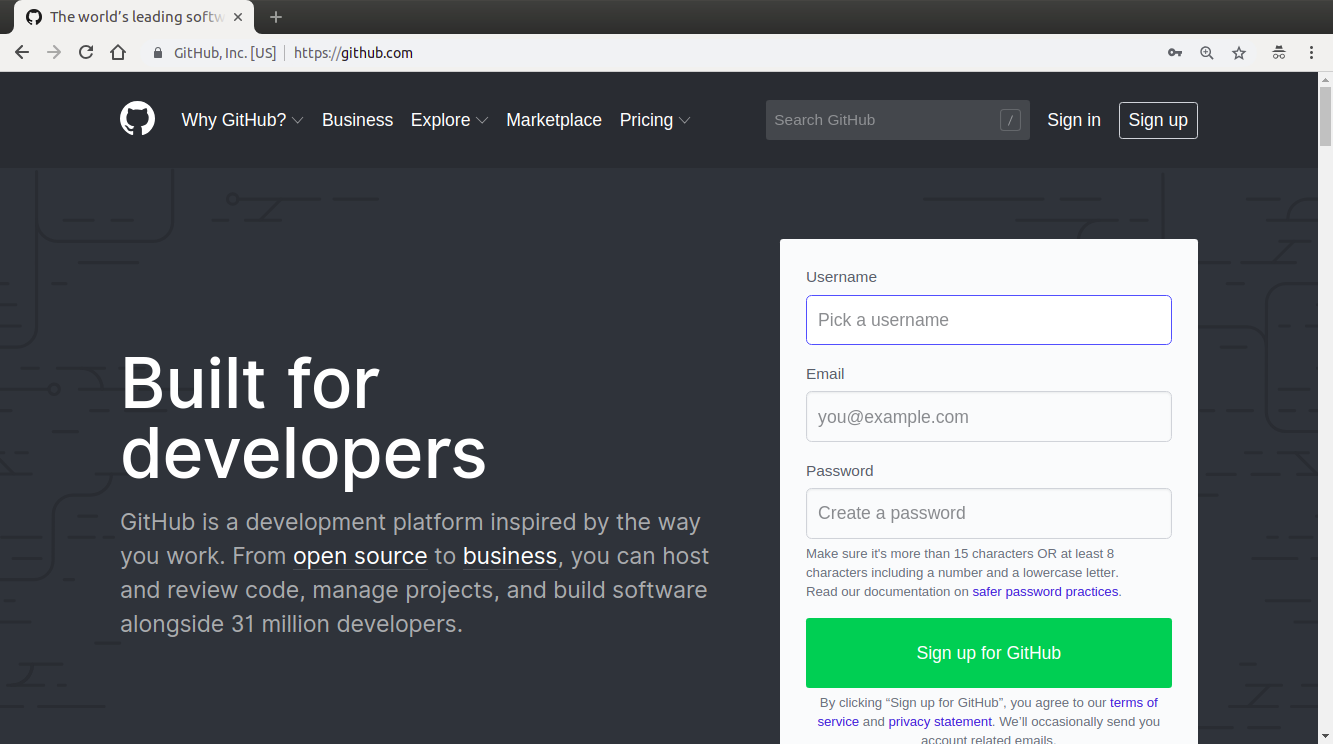
\includegraphics[width=4in]{\thischapterpath/figures/github1.png}}
  \subfigure[]
{
\includegraphics[width=4in]{\thischapterpath/figures/github2.png}}
\caption{(a) {\tt github} website. (b) Students and teachers can apply for free repositories.}
\label{fig:github12}
\end{figure}

Signing up in {\tt github} is easy, as shown in
Figure~\ref{fig:github34} (a).  After creating an account, a
repository can be created as shown in Figure~\ref{fig:github34} (b).
This website has many options: the name of the repository, whether it
is public or private, whether to initialize the repository with {\tt
  README}, etc.


\begin{figure}[h] \centering
 \subfigure[]
{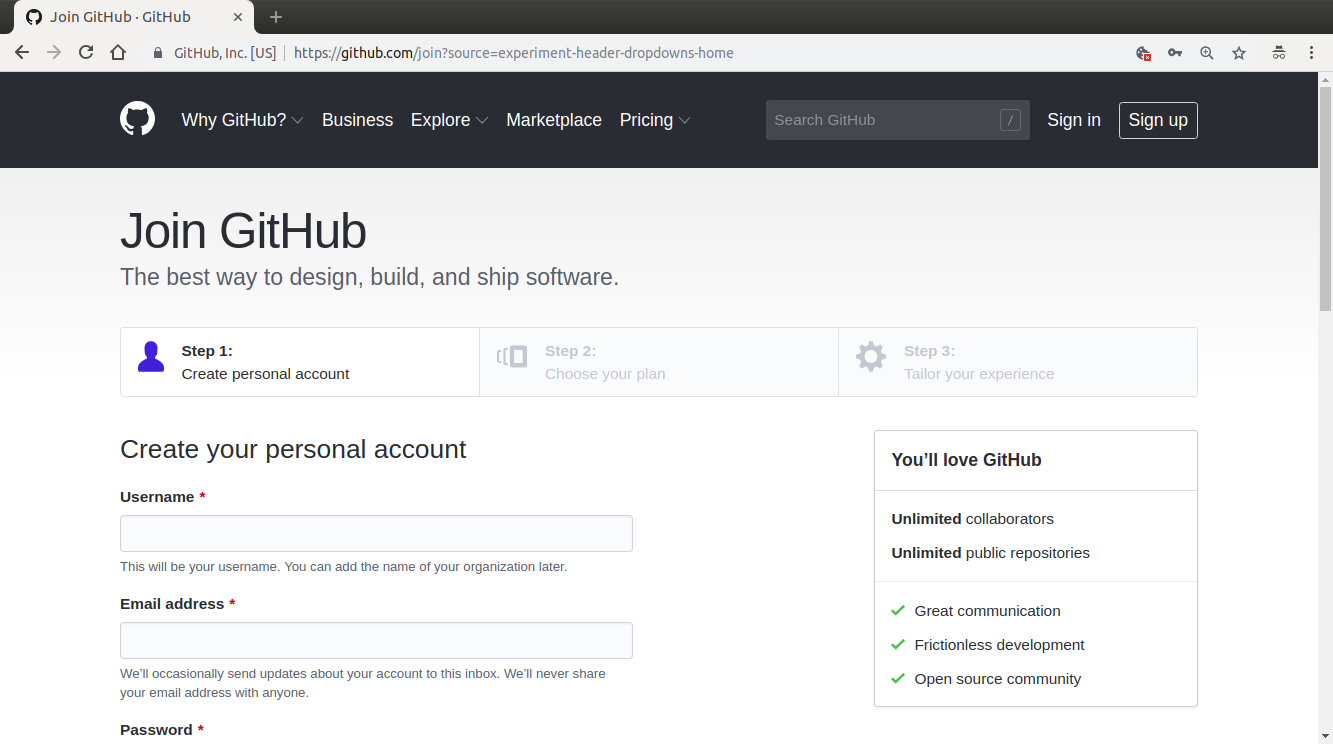
\includegraphics[width=4in]{\thischapterpath/figures/github3.png}}
  \subfigure[]
{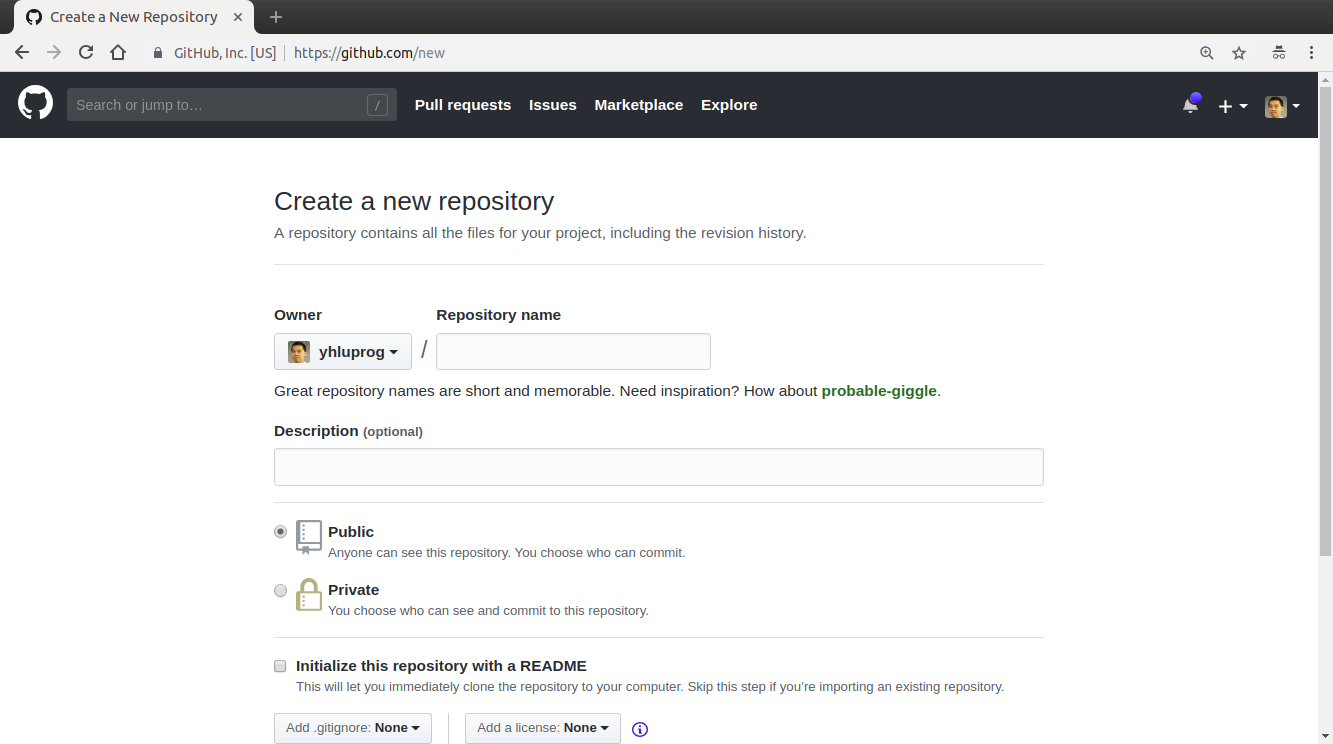
\includegraphics[width=4in]{\thischapterpath/figures/github4.png}}
\caption{(a) Create an account in {\tt github}. (b) Create a
  repository.}
\label{fig:github34}
\end{figure}

\begin{figure}[h] \centering
   \subfigure[]
{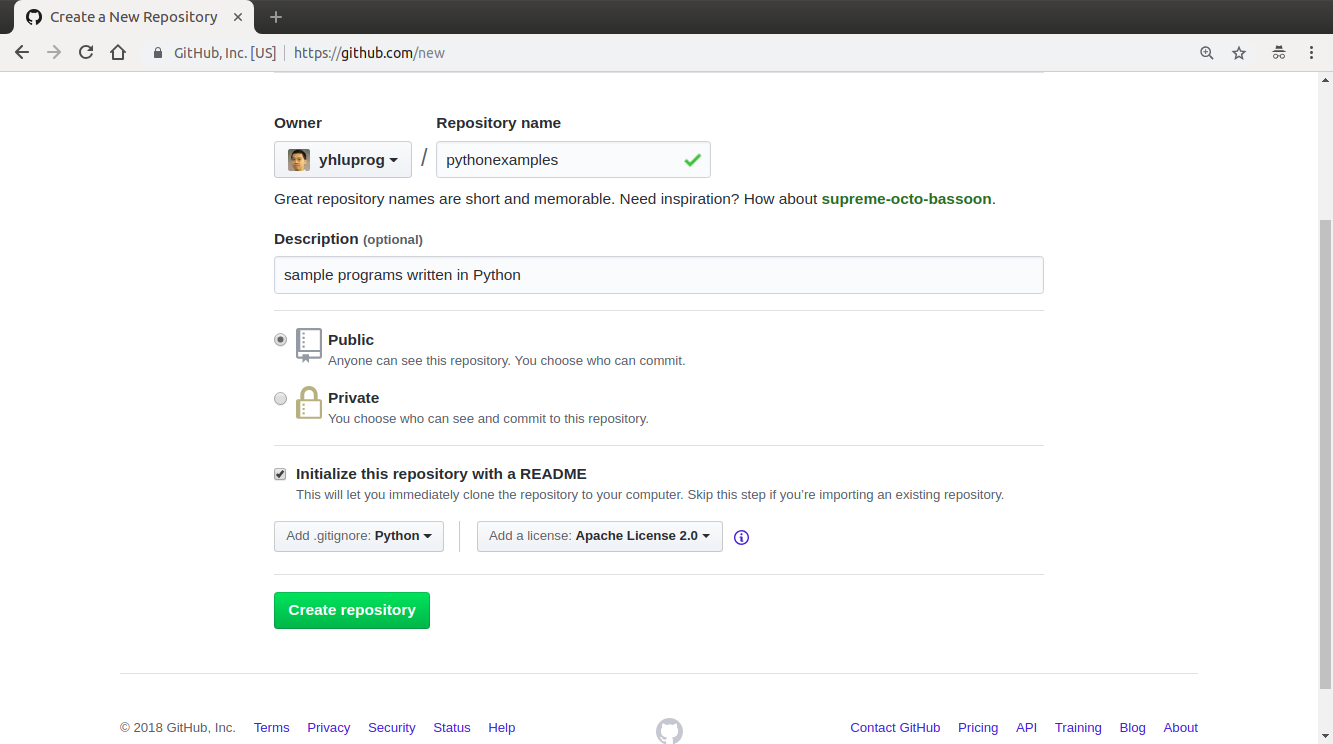
\includegraphics[width=4in]{\thischapterpath/figures/github5.png}}
   \subfigure[]
{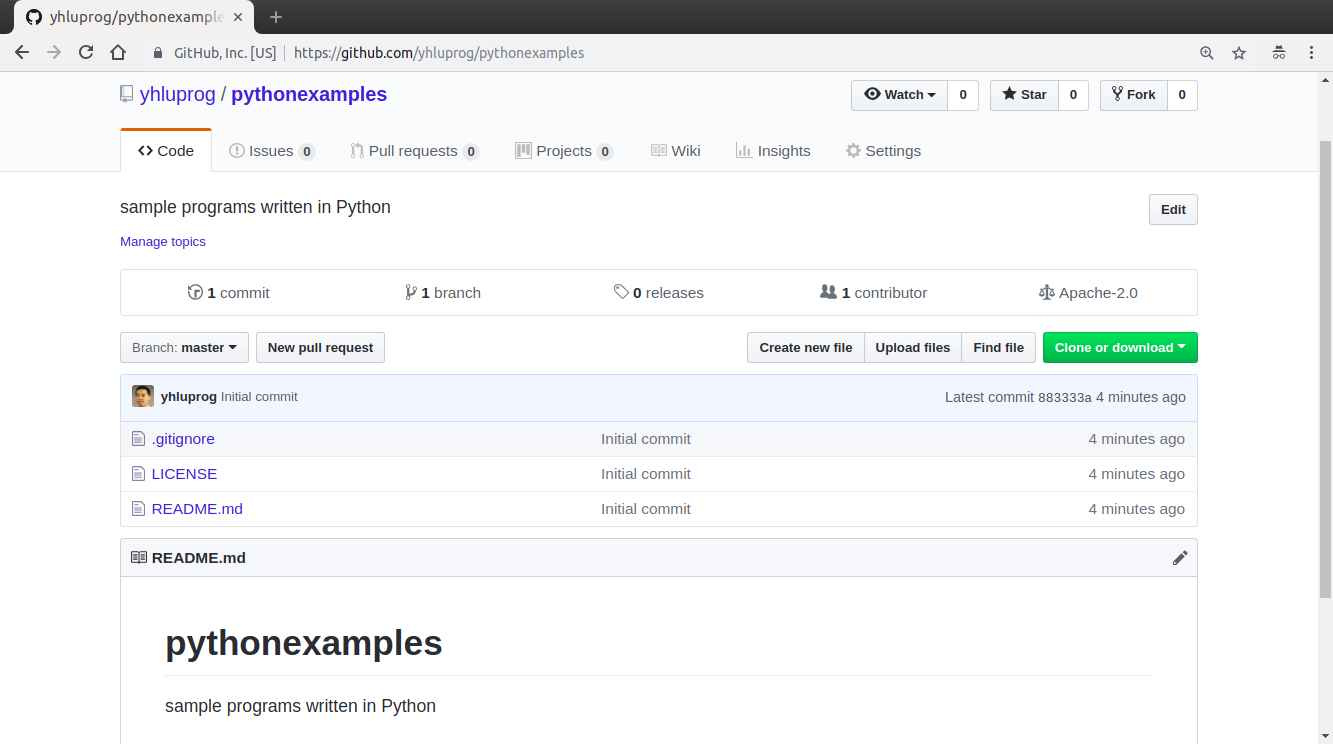
\includegraphics[width=4in]{\thischapterpath/figures/github6.png}}
\caption{(a) A new repository. (b) The repository has been created.}
\label{fig:github56}
\end{figure}

\marginnote{Is {\tt git} case sensitive? The correct answer
  is ``it is complicated''. A short answer is ``No'': you
  should treat {\tt git} as case insensitive. Do not have two
files whose names are different by cases only.}

Figure~\ref{fig:github56} (a) shows the options for creating a new repository:


\begin{itemize}
\item Repository name: pythonexamples
\item Description: sample programs written in Python
\item Public
\item Check ``Initialize this repository with a README''
\item Select ``Add .gitignore: Python''
\item Select ``Add a license: Apache License 2.0''
\end{itemize}


Figure~\ref{fig:github56} (b) shows the repository after it has been
created.  As can be seen on the website, there are many options
changing this repository.  For example, it is possible adding new
files or uploading files. It is also possible editing an file by
clicking the pen icon.

\section{Clone a Repository}

A more common way of using a repository, however, is to {\it clone} the
repository on another computer, as illustrated in Figure~\ref{fig:gitclone}.

\begin{figure}[h] \centering
{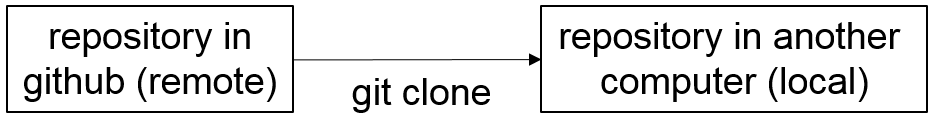
\includegraphics[width=3in]{\thischapterpath/figures/gitclone.png}}
\caption{Using {\tt git clone} command creates a repository on another computer.}
\label{fig:gitclone}
\end{figure}

To clone a repository, it is necessary knowing the {\it path} in {\tt
  github}.  Figure~\ref{fig:github7} shows the path of the repository.

\begin{figure}[h] \centering
{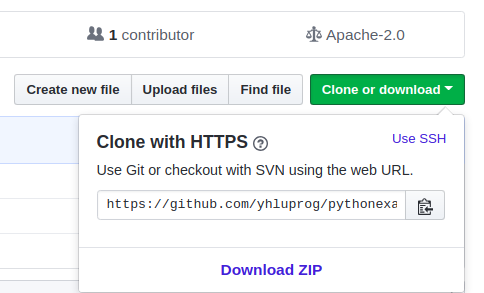
\includegraphics[width=3in]{\thischapterpath/figures/github7.png}}
\caption{Cloning a repository may use HTTPS or SSH.}
\label{fig:github7}
\end{figure}


\clearpage

To clone the repository, starts a {\it Terminal} in Linux
and type the {\tt git clone} command. In the following
example, {\tt \$} is the {\it command prompt} for the Terminal.

\vspace{0.2in}

\noindent
\begin{tabular}{|p{5in}|}\hline
\begin{verbatim}
$ git clone https://github.com/yhluprog/pythonexamples.git
\end{verbatim}
\\ \hline
\end{tabular}
\vspace{0.2in}

The command clones the repository and the following message is shown:

\vspace{0.2in}

\noindent
\begin{tabular}{|p{5in}|}\hline
\begin{verbatim}
Cloning into 'pythonexamples'...
remote: Enumerating objects: 5, done.
remote: Counting objects: 100% (5/5), done.
remote: Compressing objects: 100% (5/5), done.
remote: Total 5 (delta 0), reused 0 (delta 0), pack-reused 0
Unpacking objects: 100% (5/5), done.
Checking connectivity... done.
\end{verbatim}
\\ \hline
\end{tabular}
\vspace{0.2in}

After cloning the repository, a directory (also called folder) with
the name {\tt pythonexamples} is created.  This can be shown
using the {\tt ls} command:

\vspace{0.2in}

\noindent
\begin{tabular}{|p{5in}|}\hline
\begin{verbatim}
$ ls
pythonexamples/
\end{verbatim}
\\ \hline
\end{tabular}
\vspace{0.2in}

Inside this directory, there are already two files: {\tt
  LICENSE} and {\tt README.md}. The is a hidden file {\tt .gitignore}.
It is hidden because it starts with {\tt .} and is not shown by the
{\tt ls} command. To show a hidden file, it is necessary using the
{\tt ls -a} command. Additionally, a hidden directory (ending with
{\tt /}) called {\tt .git} is also shown.

\vspace{0.2in}

\noindent
\begin{tabular}{|p{5in}|}\hline
\begin{verbatim}
$ cd pythonexamples/
$ ls -a
./  ../  .git/	.gitignore  LICENSE  README.md
\end{verbatim}
\\ \hline
\end{tabular}
\vspace{0.2in}

Enter the directory using the {\tt cd} command
and use the {\tt ls} command to see the files and directories.

\vspace{0.2in}

\noindent
\begin{tabular}{|p{5in}|}\hline
\begin{verbatim}
$ cd .git
$ ls
branches/  config  description	HEAD  hooks/  index  
info/  logs/  objects/  packed-refs  refs/
\end{verbatim}
\\ \hline
\end{tabular}
\vspace{0.2in}


Among them, {\tt config} stores the information about
the remote repository.  The {\tt more} command can show
the content of the file:

\vspace{0.2in}

\noindent
\begin{tabular}{|p{5in}|}\hline
\begin{verbatim}
$ more config
[core]
	repositoryformatversion = 0
	filemode = true
	bare = false
	logallrefupdates = true
[remote "origin"]
	url = https://github.com/yhluprog/pythonexamples.git
	fetch = +refs/heads/*:refs/remotes/origin/*
[branch "master"]
	remote = origin
	merge = refs/heads/master
\end{verbatim}
\\ \hline
\end{tabular}
\vspace{0.2in}

The line starting with {\tt url} is the path used in {\tt git clone}.
The concept of {\it branch} will be explained later in this chapter.

\section{Commit and Push}

\marginnote{Modifying {\tt LICENSE} is not recommended.}

There are many different methods modifying a repository.  The first
method modifies an existing file.  Use a text editor and add the
following line to {\tt README.md}:

\begin{verbatim}
This repository demonstrates how to use commit, push, and branch.
\end{verbatim}

After adding this line, use the {\tt git commit} command to show which file
has been changed:

\vspace{0.2in}

\noindent
\begin{tabular}{|p{5in}|}\hline
\begin{verbatim}
$ git commit
On branch master
Your branch is up-to-date with 'origin/master'.
Changes not staged for commit:
	modified:   README.md
\end{verbatim}
\\ \hline
\end{tabular}
\vspace{0.2in}

What does this mean? It says a file {\tt README.md} has been changed
but it has not been committed. The next question is the difference
between changes and commit.  Modifications are often reviewed and
revised multiple times; these changes are transient and do not need to
be recorded in the repository.  When the modifications are
satisfactory, the file is ready to ``take a snapshot'' by creating a
new version.  The command to take a snapshot is {\tt git commit}.

The earlier {\tt git commit} shows the candidate(s) for commit.  A
candidate can be a files that has been modified ({\tt README.md} in
this example).  This command has not committed any changes yet and has
not created a new version.

\newpage

\renewcommand{\thischapterpath}{\thispartpath/test}
\chapter{Testing}


Have you ever had a situation when your software has a bug but it is
not discovered for a long time?  The existence of the bug and its
ability to escape detection may surprise your entire team. ``How did
that happen?'', you may ask.  This may happen due to a wide variety of
reasons. One of the possible reasons is that the software has not been
well tested and as a result the bug is not detected. Testing is an
important method detecting bugs.  However, testing can be tideous.  It
is common that someone makes a ``small'' change and skips testing.
The person believes the change is so small and cannot possibly have
any bug.  If several people add a few small changes here and there,
the software soon is full of ``small'' bugs.  Why do people not test
their programs immediately after they have made changes?  One reason
is that testing require additional work.

Is it possible testing is fully automated without any additional
effort? {\it Continuous Integration} (CI) does exactly that.

You still need to write testers. There is no way avoiding that part.
What continuous integration does is to automatically invole these
testers whenver you push your program to the shared repository.
This chapter uses {\tt Travis-CI} for continuous integration. Before explaining how
to use Continuous Integration, it is necessary first explaining how Python
testing works.

\section{Limitations of Testing}

It is important understanding that testing has limitations.  It is
practically impossible testing every possible scenario.  Every {\tt
  if} is a {\it condition}. A condition divides a program into two
different paths depending whether the condition is true or not.  A
non-trivial program can easily have hundreds of conditions.  As a
simple explanation why it is not possible testing every possible
scenario. Let's consider a program with 100 {\it independent}
conditions, i.e., whether condition is true or false does not affect
any other condition.  There are $2^{100}$ possible scenarios.  The
fastest computer in the world can perform several hundred quadrillion
($10^{15}$) calculations per second; this is a parallel computer but
let's not worry about that detail.  Because $\log_2(10) \approx 3.3$,
$10^{15} \approx 2 ^ {50}$. Thus, the fastest computer can check as
many as $2 ^ {50}$ conditions per second. How many can this computer
check per minute? $2 ^ {50} \times 60$. How about a day (86,400
seconds)?  $2 ^ {50} \times 86400 \approx 2 ^ {66}$.  In order to test
$2^{100}$ possible scenarios, this computer needs to work $2^{34}$
days; this is very long time (much longer than the history of humans).
In fact, the situation is even worse.  The estimation above considers
only two possible cases for each condition: true or false. If the
condition compares two numbers, then ``every possible scenario'' means
every possible pairs of these two numbers.  What does this mean? It
would be completely impossible testing every possible scenario of a
program's execution paths controlled by the conditions.

Does this mean there is no need to test because it is not possible
testing all possible scenarios? No. What it means is that testing has to
be done carefully so that testing can detect as many problems (i.e.,
bugs) as possible.  Good tests should consider many different scenarios.

\section{Structure of Tests}

Many books talk about the importance of testing and how to write
tests.  However, few books talk about how to structure tests. Before
writing any test, you need to answer an important question: do you
want the testing code to be sent to the users (or customers)? In most
cases, the answer is no.  The program used to generate the product
sent to customers is often called the ``production code''.  You do not
want to include test code inside production code for many reasons.
First, including testing code may make your product bigger (in terms
of storage) and slower (in terms of execution time). Worse, testing
often needs specific inputs and the expected outputs for these test
cases.  Will you also give these inputs and outputs to your customers?
If you do not, why do you include testing code in the product?

Mixing production code and testing code is a common mistake for
beginning software developers. Worse, many of them have a lot of
``debugging messages'' as they test  code. When the program is
ready for production and release, what will they do with these
debugging messages?  In almost all cases, your customers do not
understand the debugging messages and you have to remove the code
printing these messages.  Here is the problem. When you remove the
code printing these messages, the risk is too high for one of two
things to happen. First, you do not remove all the code printing the
debugging messages.  Your customers are annoyed by the mysterious
debugging messages. Your competitors know more than what you to reveal
about your proudct.  The second scenario is worse.  You accidentally
remove more code than you intend and you actually add bugs to your
program.  Your program no longer works and your customers are very
angry at your product.

The correct way of creating tests is to separate testing code from the
production code in different files (probably in different
directories).  The production code does what it needs to do
as the product. The
testing code tests the production code.  When your product is ready,
exclude the testing code, the inputs, and the expected outputs before
releasing your product.  Figure~\ref{fig:teststructure01} illustrates
this concept.

\begin{figure}[h] \centering
{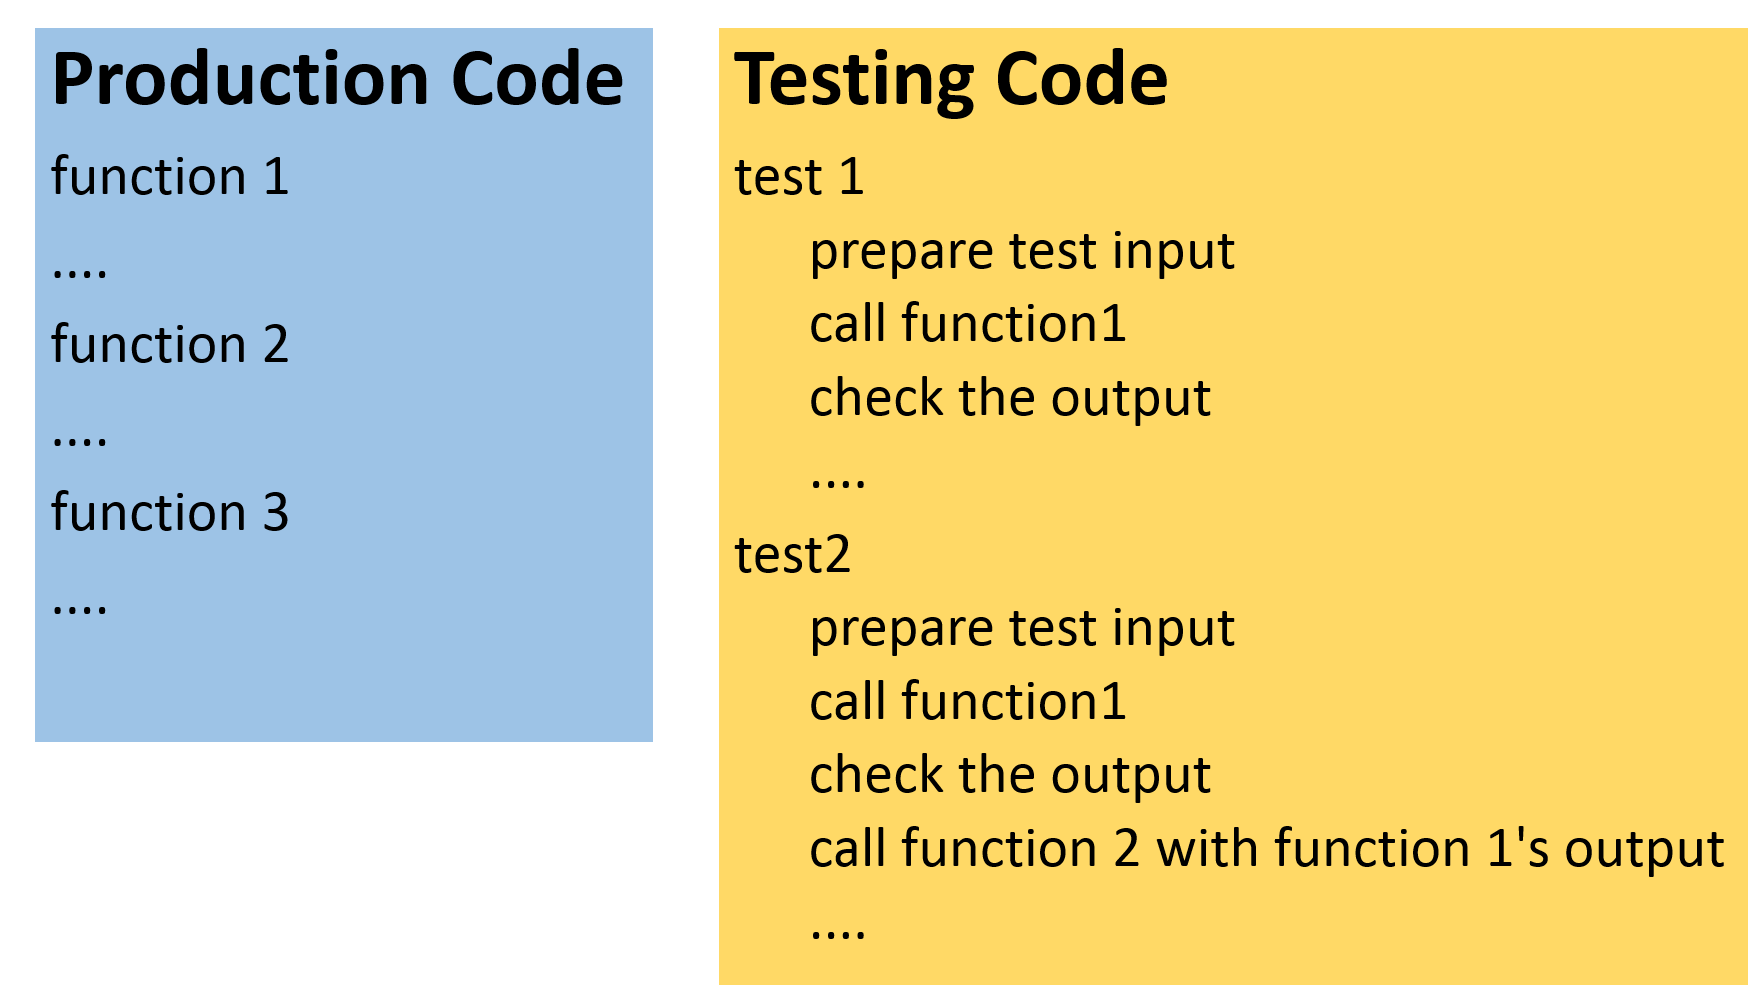
\includegraphics[width=4.5in]{\thischapterpath/figures/teststructure01.png}}
\caption{Production code and test code should be completely separated.}
\label{fig:teststructure01}
\end{figure}

\index{assert|(}
\section{Use {\tt Assert} Correctly}

Another common mistake among beginning software developers is to use
{\tt assert} incorrectly. This is what they often do.

\marginnote{These problems about misuse {\tt assert} were observed
  in the authors' classes.  They actually happened multiple times.}

\vspace{0.2in}

\noindent
\begin{tabular}{|p{5in}|}\hline
\begin{verbatim}
  # This is production code
  ....
  assert(condition that should be true)
  ....
\end{verbatim}
\\ \hline
\end{tabular}
\vspace{0.2in}

This is one example how {\tt assert} may be used:

\vspace{0.2in}

\noindent
\begin{tabular}{|p{5in}|}\hline
\begin{verbatim}
def func(x):
    assert (x > 1)
\end{verbatim}
\\ \hline
\end{tabular}
\vspace{0.2in}

There are three problems when you do this.  First, if the condition is
not true, the program {\it immediately} stops.  There is no second
chance.  Imagine that your program is a text editor. When a user wants
to save the content to a file, your program does not want to erase an
existing file.  You put {\tt assert} there claiming that the file must
not exist. If a user accidentially uses a file whose name already
exists, the program stops and everything typed by the user is lost.
You will definietely have a user that will never buy any product from
you.  Some people argue that ``I put {\tt assert} there because I know
it must be true.'' That argument is self-contraditory.  If you know
that the condition must be true, you will not put {\tt assert} there.
Would you write

\vspace{0.2in}

\noindent
\begin{tabular}{|p{5in}|}\hline
\begin{verbatim}
assert (1 > 0)
\end{verbatim}
\\ \hline
\end{tabular}
\vspace{0.2in}

You don't.

If you are abosolutly certain the condition must be true, you do not
need to put {\tt assert} there.

Some people say, ``I will remove all {\tt assert} before releasing the
product.''  This can be done easily using the {\tt grep -v} command.
This, however, brings the second problem.  What would happen if
some of the {\tt assert} statements actually do something useful?
Consider the following case:

\index{grep}


\vspace{0.2in}

\noindent
\begin{tabular}{|p{5in}|}\hline
\begin{verbatim}
assert (x = y)
\end{verbatim}
\\ \hline
\end{tabular}
\vspace{0.2in}

This assigns {\tt y}'s value to {\tt x}.

What you really want to do is probably to ensure that  {\tt x} and {\tt y}
are the same:

\vspace{0.2in}

\noindent
\begin{tabular}{|p{5in}|}\hline
\begin{verbatim}
assert (x == y)
\end{verbatim}
\\ \hline
\end{tabular}
\vspace{0.2in}

The earlier {\tt assert} statement assigns {\tt y}'s value to {\tt
  x}. Hence, their values are same and the intended {\tt assert} is
actually true.  If you remove the {\tt assert} and no longer assign
{\tt y}'s value to {\tt x}, the program may not work any more. Human
eyes are not good detecting the differences between {\tt =} and {\tt
  ==}. This is a difficult bug to fix because keeping {\tt assert}
means the program is correct. Removing {\tt assert} means the program
is wrong.


\marginnote{Do not put {\tt assert} in your production code.}

The third problem is, perhaps, somewhat philosophical.  It is the
attitude of creating good software.  Software is deployed in many
safety-critical systems. Mistakes in these systems may cause
signficant amounts of financial losses, body injuries, or even deaths.
Allowing a program to sudden stop is simply an unacceptable way of
thinking.  Using {\tt assert} is an {\it irresponsible} way of writing
production code.  It expresses the attutide ``Something is not
expected. My program commits suicide and the rest is not my problem
any more.''  A more responsbile way of writing good software is to
{\it handle the problem and do not stop the program}.

If {\tt assert} has these problems, does that mean {\tt assert} should
not be used at all?  You should not use {\tt assert} in production
code.  You can use {\tt assert} in the testing code, as shown in
Figure~\ref{fig:teststructure02}.


\begin{figure}[h] \centering
{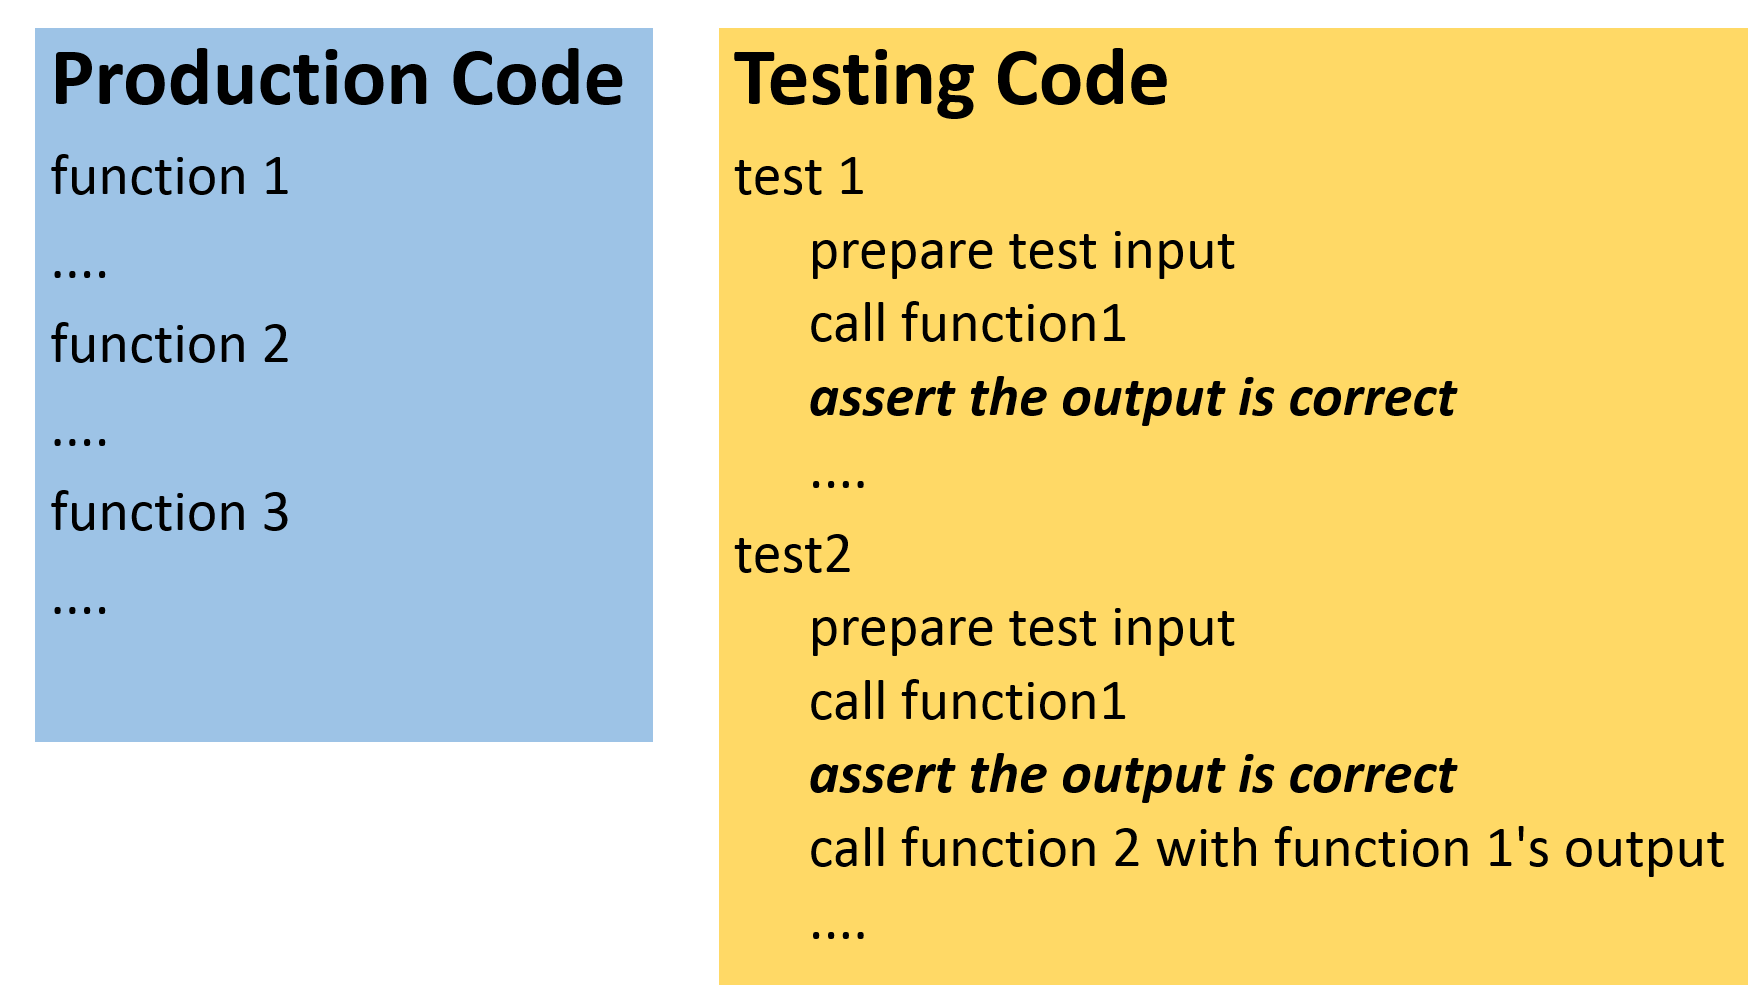
\includegraphics[width=4.5in]{\thischapterpath/figures/teststructure02.png}}
\caption{Use {\tt assert} in the testing code.}
\label{fig:teststructure02}
\end{figure}

In this example, the testing code uses {\tt assert} to check whether
the output from function 1 is correct.  This is particularly important
before sending it to the input of function 2.  This further emphasizes
the importance of separating production code from testing code.

\index{assert|)}

\section{Exception}

\index{pytest|(}
\section{Pytest}

Python has a tool for testing calle {\tt pytest}. It automatically
looks for the files starting with {\tt test\_} and ending with {\tt
  .py} and executes the functions whose names start with {\tt test\_}.
The following is a simple example.


\resetlinenumber[1]
\linenumbers
\begin{tt}
  \lstinputlisting{\progpath/software/test/test_example1.py}
\end{tt}
\nolinenumbers

Running {\tt pytest} gets the following output:

\vspace{0.2in}

\noindent
\begin{tabular}{|p{5in}|}\hline
\begin{verbatim}
$ pytest
============ test session starts =============
platform linux -- Python 3.5.2, pytest-4.3.0, py-1.8.0, pluggy-0.9.0
rootdir: /..., inifile:
collected 1 item

test_example1.py .                                
\end{verbatim}
\\ \hline
\end{tabular}
\vspace{0.2in}

Here, the {\tt rootdir} is the directory where you run {\tt pytest}.
This output means the tests have passed.

Change the program  as follows: {\tt returntrue} returns {\tt False}
and {\tt returnfalse} returns {\tt True}:

\resetlinenumber[1]
\linenumbers
\begin{tt}
  \lstinputlisting{\progpath/software/test/test_example2.py}
\end{tt}
\nolinenumbers

Running {\tt pytest} gets this result, showing the test has failed.


\vspace{0.2in}

\noindent
\begin{tabular}{|p{5in}|}\hline
\begin{verbatim}
======================== FAILURES ========================
____________________ test_truefalse ______________________

    def test_truefalse():
>       assert returntrue() == True
E       assert False == True
E        +  where False = returntrue()

test_example2.py:11: AssertionError
==================== 1 failed in 0.04 seconds ====================
\end{verbatim}
\\ \hline
\end{tabular}
\vspace{0.2in}

\marginnote{A test is useless if it can never fail.}

When you create tests, it is important that you check whether the
tests may fail. Passing tests is not the purpose of testing.  The
purpose of testing is to detect mistakes in production code and
correct the code.  If a test can never fail, this test is useless.

Next, considers a slightly more complex program for testing two
functions: {\tt f1} and {\tt f2}:

\resetlinenumber[1]
\linenumbers
\begin{tt}
  \lstinputlisting{\progpath/software/test/test_example3.py}
\end{tt}
\nolinenumbers

This is the output of {\tt pytest}:

\vspace{0.2in}

\noindent
\begin{tabular}{|p{5in}|}\hline
\begin{verbatim}
======================== FAILURES ========================
_______________________ test_f1f2 ________________________

    def test_f1f2():
        assert f1(3) == 4
        assert f1(-3) == -2
>       assert f2(3) == 4
E       assert 2 == 4
E        +  where 2 = f2(3)

test_example3.py:13: AssertionError
\end{verbatim}
\\ \hline
\end{tabular}
\vspace{0.2in}

The result says that calling {\tt f1(3)} and {\tt f1(-3)} have passed
the tests. Calling {\tt f2(3)} has failed because {\tt f2(3)}
return 2 but the test program expects 4.

Earlier this chapter said testing code and production code should be
separated. The examples for {\tt pytest} above violated this rule.
The following examples will follow the rule separating the testing
code from the tested code. Consider a file with two functions: {\tt
  f1} and {\tt f2}:

\resetlinenumber[1]
\linenumbers
\begin{tt}
  \lstinputlisting{\progpath/software/test/funcs.py}
\end{tt}
\nolinenumbers

This is the output when calling the functions interactively:

\vspace{0.2in}

\noindent
\begin{tabular}{|p{5in}|}\hline
\begin{verbatim}
$ python3
Python 3.5.2 (default, Nov 12 2018, 13:43:14) 
[GCC 5.4.0 20160609] on linux
Type "help", "copyright", "credits" or "license" for more information.
>>> import funcs
>>> funcs.f1(3)
4
>>> funcs.f2(5)
6
25
15
\end{verbatim}
\\ \hline
\end{tabular}
\vspace{0.2in}

A test program calls {\tt funcs.f1(3)} and {\tt funcs.f2(5)}.

\resetlinenumber[1]
\linenumbers
\begin{tt}
  \lstinputlisting{\progpath/software/test/test_example4.py}
\end{tt}
\nolinenumbers

Running {\tt pytest}, however, has no output. What is happening?
Instead of printing to a computer screen (also called the {\it
  console}), {\tt pytest}, captures the output.  The reason is that
{\tt pytest} does not want to print too many things.  If too many
things are printed to the screen, it is likely that some important
messages are ignored. Another reason is that {\tt pytest} often runs
automatically when no human is watching (more details about this
later in the section on Continuous Integration).
There are two solutions: The first is to tell
{\tt pytest} to print to the screen by adding {\tt -s} after {\tt
  pytest}.  This defeats the purpose of {\tt pytest}'s intention not
to print to the screen.

\index{pytest|-s}

The second is a better and more general solution: it saves the
captured output to a file. It is actually quite straightforward:

\resetlinenumber[1]
\linenumbers
\begin{tt}
  \lstinputlisting{\progpath/software/test/test_example5.py}
\end{tt}
\nolinenumbers

\index{console}

The function {\tt test\_f1f2) has an input for capturing the outputs.
  This input will be provided automatically by {\tt pytest}.  To get
  the captured output, it calls {\tt readouterr()}.  This function
  returns the captured output to standard output (also called {\tt
    stdout}) and the standard error (also called {\tt stderr}).
  Separating {\tt stdout} from {\tt stderr} gives more flexibility:
  the former is the normal output and the latter is the error
  messages.  By default, both {\tt stdout} and {\tt stderr} are shown
  on a computer screen but it is possible saving them to different
  files.

  The testing program {\tt test\_example5.py} saves the standard
  output to a file called {\tt capturedstdout}. All outputs by the
  {\tt print} statements in {\tt funcs} are saved in this file.
  The content of the file is (as expected)

 
\vspace{0.2in}

\noindent
\begin{tabular}{|p{5in}|}\hline
\begin{verbatim}
4
6
25
15
\end{verbatim}
\\ \hline
\end{tabular}
\vspace{0.2in}

When the outputs are saved to a file, testing can be done automatically
without human watching by following these steps:

\begin{enumerate}[noitemsep,nolistsep]
\item write the expected output to a file
\item capture the output from {\tt pytest} and save it to another file
\item compare the two files
\end{enumerate}

The following program shows these steps

\resetlinenumber[1]
\linenumbers
\begin{tt}
  \lstinputlisting{\progpath/software/test/test_example6.py}
\end{tt}
\nolinenumbers

The tests uses {\tt filecmp.cmp} to compare the context of two files.
As explained, if a test cannot fail, it is useless. If {\tt
  funcs.f2(5)} is replaced by {\tt funcs.f2(4)}, {\tt pytest} fails.
This suggests that {\tt pytest} is actually testing {\tt funcs.f2}.

\section{Test Integer Partition}

Only ``toy'' examples for {\tt pytest} are shown so far.  By capturing
the outputs, {\tt pytest} can compare expected outputs with the actual
outputs.  Thus, it becomes much easier testing many cases using a
single test program. The following program tests integer partition
using three different values: 3, 4, and 5. The expected outputs are
stored in a separate directory called {\tt expected} and the files are
called, not surprisingly, {\tt 3}, {\tt 4}, and {\tt 5}.

\resetlinenumber[1]
\linenumbers
\begin{tt}
  \lstinputlisting{\progpath/software/test/test_intpart1.py}
\end{tt}
\nolinenumbers

\section{Test Coverage}

\index{test coverage}
\index{coverage}
\index{coverage!run}
\index{coverage!annotate}


{\it Test coverage} means how much percentage of code that has been
tested.  Getting test coverage is pretty easy: python has a program
called {\tt coverage}. Simply adding {\tt coverage run} before the
program to be tested (and the necessary arguments).


\vspace{0.2in}

\noindent
\begin{tabular}{|p{5in}|}\hline
\begin{verbatim}
$ coverage run intpart.py -e -o 5
-e and -o cannot be both set
$ coverage report
Name         Stmts   Miss  Cover
--------------------------------
intpart.py      50     26    48%
\end{verbatim}
\\ \hline
\end{tabular}
\vspace{0.2in}

The first {\tt coverage run} command executes the Python program {\tt
  intpart.py} with arguments {\tt -e -o 5}.  Since it is not possible
partitioning any integer using only even numbers and using only odd
numbers at the same time, the {\tt intpart.py} program stops without
partitioning the input value 5. The coverage is 48\%.

To see which line has been tested, add {\tt annotate}
after {\tt coverage} and the file {\tt intpart.py,cover}
is created, as shown below

\resetlinenumber[1]
\linenumbers
\begin{tt}
  \lstinputlisting{\progpath/software/test/intpart.py,cover1}
\end{tt}
\nolinenumbers

If a line starts with {\tt >}, this line has been tested.
If a line starts with {\tt !}, this line has not been tested.

Next, run {\tt intpart.py} again without {\tt -e} or
{\tt -o}.  This time {\tt coverage report}
says 80\% code is covered and {\tt coverage annotate}
generates the following file:

\resetlinenumber[1]
\linenumbers
\begin{tt}
  \lstinputlisting{\progpath/software/test/intpart.py,cover2}
\end{tt}
\nolinenumbers

Many lines change from {\tt !} (not tested) to {\tt >} (tested).

The second test has 80\% coverage, higher than the first test. Is a
higher coverage always better? This a common misunderstanding.  The
purpose of testing is to discover problems.  If a test can discover
problems, it is a good test even if it covers only a small percentage
of code.  The next common misunderstanding may surprise you: Even if
your tests have 100\% coverage, the program may still have undiscoverd
problems.  ``How can that be possible?'' ``100\% test coverage.''

The misunderstanding occurs from the definition of coverage.  Test
coverage is defined by whether each line has been tested; it is not
defined by whether each scenario has been tested. What is the
difference? Consider the following example:

\vspace{0.2in}

\noindent
\begin{tabular}{|p{5in}|}\hline
\begin{verbatim}

if (condition1):
    # A
else:
    # B
...
if (condition2):
    # C
else:
    # D
...
\end{verbatim}
\\ \hline
\end{tabular}
\vspace{0.2in}

The flow can be expressed in Figure~\ref{fig:twoconditions}.

\begin{figure}[h] \centering
{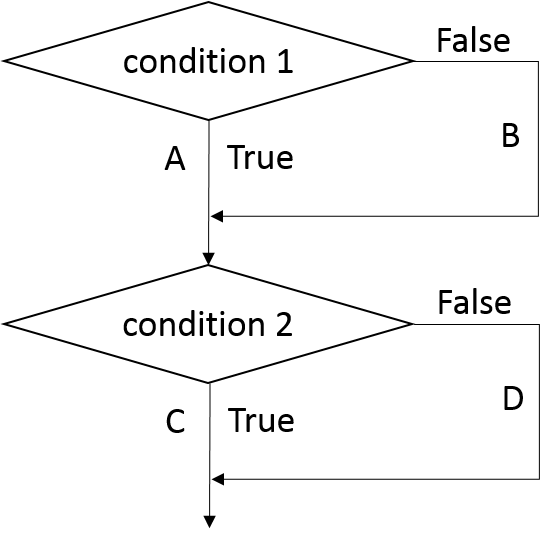
\includegraphics[width=2in]{\thischapterpath/figures/twoconditions.png}}
\caption{The flow of two conditions.}
\label{fig:twoconditions}
\end{figure}

There are four possible scenarios of the two conditions:

\begin{enumerate}[noitemsep,nolistsep]
\item condition1: True, condition2: True
\item condition1: True, condition2: False
\item condition1: False, condition2: True
\item condition1: False, condition2: False
\end{enumerate}

If a test has True for condition1 and False for condition2, then A and
D have been tested. Another test has False for condition1 and True for
condition2, then B and C have been tested.  These two test cases have
tested A, B, C, and D. In other words, all code has been tested and
the coverage is 100\%.

``Wait'' ``How can it be possible to get 100\% coverage even with only
two tests? There are four scenarios.'' You may ask.

That is the problem.

What does this mean? Does this mean coverage is not helpful? Test
coverage is very helpful.  percentage. You should check whether the
specific lines you want to test have been covered.  Do not focus on
the coverage number only.


\section{Continous Integration}

\begin{figure}[h] \centering
{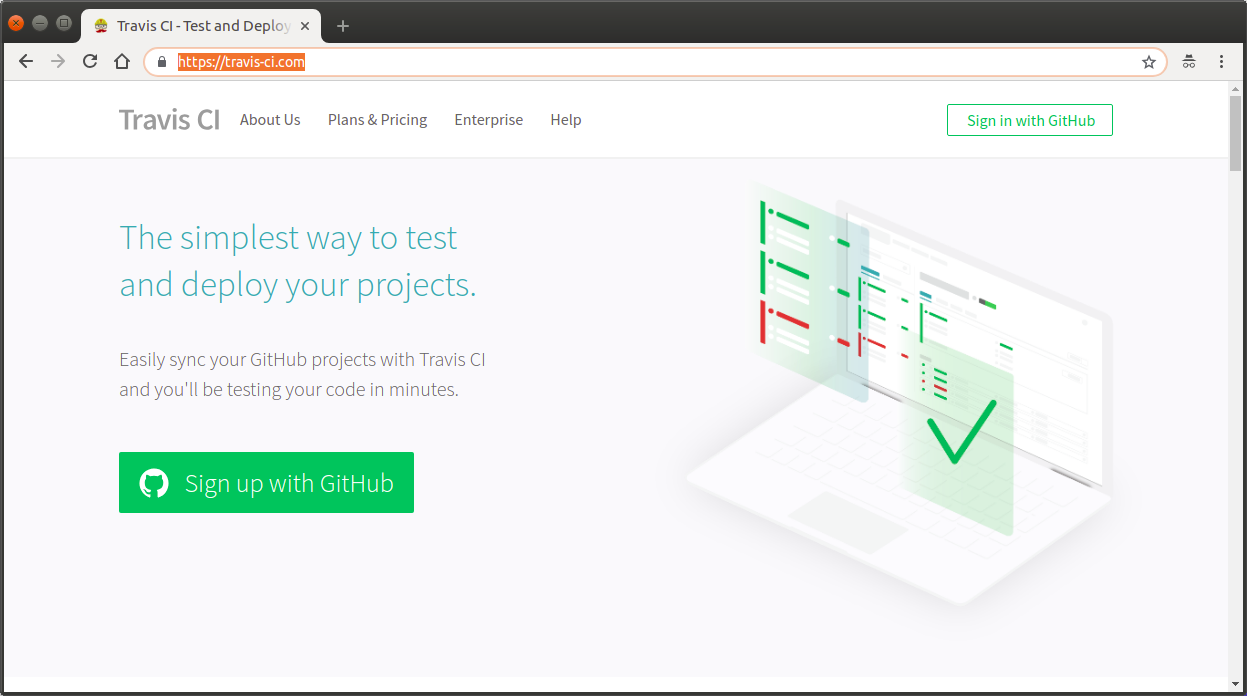
\includegraphics[width=4.5in]{\thischapterpath/figures/travis01.png}}
\caption{Travis-CI.com is a website supporting continuous integration.}
\label{fig:travis01}
\end{figure}

\index{pytest|)}

\newpage

\renewcommand{\thischapterpath}{\thispartpath/ws}
\chapter{Web Services}

\newpage

\renewcommand{\thischapterpath}{\thispartpath/graphics}
\chapter{Graphics/Visualization}

\newpage





\begin{comment}
Part 2: Machine Learning I: Unsupervised Learning (mathematics)
   Chapter 6: k-mean
   Chapter ?: Floating Point
   Chapter 7: Hierarchical Clustering
   Chapter 8: Support vector machines
\end{comment}

\newcommand{\unsuppath}{\basepath/unsupervised}

\part{Machine Learning}

\chapter{Machine Learning}



\section{Learning Objectives}


\begin{itemize}
\item Understand the strength and limitations of machine learning
\item Distinguish  unsupervised learning,  supervised learning,  reinforcement learning, and transfer
  learning
\end{itemize}

\section{Decision Problems}

\index{decision problem}


\subsection{Bring an Umbrella or not?}

Machine learning means using computer programs to discover patterns
(i.e., ``learn'') from data. How is this different from typical
computer programs?  Let us consider a {\it decision problem}:
Should you bring an umbrella or not?  This should be easy, right?


\begin{verbatim}
If it is raining then
   Bring an umbrella
Otherwise
   

% YHL: I have problems using 
% \usepackage{algorithmic} or
% \usepackage[linesnumbered,ruled,vlined]{algorithm2e}
\end{verbatim}

This is simple enough.  If you always follow this rule, you will soon
encounter situations when this rule is not good.  Maybe it is not raining
right now but it is expected to rain soon. Thus, you add one more rule:

\begin{verbatim}
If it is raining then
   Bring an umbrella
Otherwise
   If it is expected to rain soon then
      Bring an umbrella
   Otherwise
      Do not bring an umbrella
\end{verbatim}



If you follow these rules, you will soon discover that they are still
insufficient.  If you are going to walk in covered areas (such as
subway stations or shopping malls), maybe you do not need an umbrella.
Thus, you add another rule:

\begin{verbatim}
If it is raining and you will walk outside covered areas then
   Bring an umbrella
Otherwise
   If it is expected to rain soon and walk outside covered areas then
      Bring an umbrella
   Otherwise
      Do not bring an umbrella
\end{verbatim}

If you are carrying a box and it does not rain heavily, maybe you
do not want to take an umbrella because it is inconvenient to carry
the box and to hold an umbrella at the same time. As a result,
the rules become

\begin{verbatim}
If it is raining and you will walk outside covered areas then
   If carrying a box and the rain is light then
       Do not bring an umbrella
   Otherwise
       Bring an umbrella
Otherwise
   If it is expected to rain soon and walk outside covered areas then
      Bring an umbrella
   Otherwise
      Do not bring an umbrella
\end{verbatim}

The rules become more and more complex.  You may also want to consider
whether it is windy. If it is, you may want to wear a raincoat instead
of bringing an umbrella. If you want to ride a bike, you may want to
choose a rain coat instead of an umbrella.  Maybe it is very hot and
you want to walk in rain to cool.  As you can see, this decision
problem has so many different scenarios and writing all these {\tt
  if}-{\tt else} conditions becomes really complex.

\subsection{Cross a Stree Intersection?}

If you drive a car, should you cross a street intersection or not?
You may think this is really easy:

\begin{verbatim}
If the traffic light is green then
   Cross the intersection
Otherwise
   Do not cross the intersection
\end{verbatim}

Sometimes, you cannot enter the inserction because it is blocked
by vehicles already. If you enter the intersection, you will park
at the intersection and worsen traffic jam. Thus, you add another rule:

\begin{verbatim}
If the traffic light is green and the intersection is clear then
   Cross the intersection
Otherwise
   Do not cross the intersection
\end{verbatim}

If you hear the siren of an ambulance, you should allow it to pass first.
Consequently, the rule gets more complex:

\begin{verbatim}
If the traffic light is green and the intersection is clear and there is no siren then
   Cross the intersection
Otherwise
   Do not cross the intersection
\end{verbatim}

If there is a jaywalker, you don't want to hit the person. Let's add that into the rule:

\begin{verbatim}
If the traffic light is green and the intersection is not occupied 
 and no siren and no jaywalker then
   Cross the intersection
Otherwise
   Do not cross the intersection
\end{verbatim}

If there is a construction and a flagman, you should follow the
flagman's instruction, not the traffic light.  

\begin{verbatim}
If a flagman signals to cross the intersection then
   Cross the intersection
Otherwise
   If the traffic light is green and the intersection is clear 
     and no siren and no jaywalker then
       Cross the intersection
   Otherwise
       Do not cross the intersection
\end{verbatim}

We can keep adding more and more rules to cover many different
scenarios.  As you can see, this decision problem may consider many
factors and writing down these rules become increasingly complex and
difficult.

\index{mortgage}
\subsection{Approve a Mortgate Application?}

If you are a bank manager and evaluate mortgage applications, how do
you decide whether to approve or not?  If you approve the application
and the person pays regularly, your bank makes money from fees and
interests.  If the person fails to pay (called ``defaults''), the bank
may lose money. It is possible that the bank does not lose money
if the house's value is sufficient to cover the mortgage (through
foreclosure). Foreclosure can be a lengthy process and most banks want
to avoid it.  How do you decide? Maybe you decide based on the
person's regular income: \index{default} \index{foreclosure}


\begin{verbatim}
If the montly income is great than twice of the monthly payment then
   Approve the mortgate application
Otherwise
   Deny the mortgate application
\end{verbatim}

If you do this, your bank will likely lose a lot of money because you
need to consider other factors, for example, whether the person
already has a lot of debt. You probably also want to consider whether
this person has a record of failing to pay bills.  If the house is not
in a popular location, you definitely want to avoid the possibility of
foreclosure. If the person has been doing business with the bank for
several years, you would trust this person more than a new customer.
Do you want to consider whether this person already own one or more
houses?  Should you consider this person's age?  Would the marital
status affect your decision?  You may want to consider the economy as
well. If economy is strong, this applicant is likely to keep the
current job or even get a raise; thus, this applicant is likely to pay
the mortgage. If economy is weak, this applicant may lose the current
job and fails to pay.  If you want to consider many factors, are some
factors are more important than the others? How do you choose the
important factors?  This problem, again, shows that considering many
factors and writing down the rules become increasingly complex and
difficult.

\section{Decisions and Feedback}

In our everyday life, we make hundreds of decisions: what clothes to
wear, where to go for lunch, what to buy in a store, what birthday
gift to send to a friend, etc.  The previous examples show that
decision problems often need to consider many factors.  The reason we
need to consider many factors is to prevent making wrong decisions.
What are ``wrong'' decisions? If you bring an umbrella and it does not
rain, it is a wrong decision.  If you do not bring an umbrella and it
rain heavily, it is a wrong decision.  Some wrong decisions have
negligible consequences: bringing an umbrella (if it is small and
light) without using it may not be a big problem.  Some wrong
decisions can have dire consequences: approving a mortgage and it
defaults, the bank loses a lot of money, possibly 
millions of dollars.

What is a ``wrong'' decision? It may not be so obvious.  A bank may
deny all mortgage applications that have slight chances of
defaults. This may completely avoid defaults but the bank also loses
opportunities making money from the applications that may, but do not,
default.  In this case, ``preventing defaults'' and ``making money''
are two related but different goals.

After knowing the consequences of a decision, we may conclude that it
is a right or a wrong decision. This is the {\it feedback} of the
decision.  With the feedback, we hope to make better decisions in the
future. For example, if the bank approves a mortgage and it defaults,
the bank would probably deny the next application that is ``similar''
to the defaulted one.  The problem is how to determine two mortgage
applications are ``similar''.

For some problems, it is impossible (or almost impossible) to know
whether a wrong mistake has been made. Suppose you are a bank manager
and you deny a mortgage application. You will not know whether this
person would be able to pay mortgage regularly because you have denied
the application.


\index{feedback}

\section{Knowledge in Data}

\index{infer}
\index{pattern}

The examples described earlier are decision problems: whether to bring
an umbrella, whether to approve a mortgage application, etc. Each
problem needs to consider many factors and it is not clear which
factor is more than the other. One way to solve these problems is to
examine similar scenarios in the past and their results: if the
current mortgage application is ``similar'' to one that approved in
the past, was that approval a right decisoin (i.e., did not default)?
Instead of writing rules, this new approach uses past data to guide
future decisions.  This is what {\it machine learning} can be helpful:
computer programs discover (i.e., ``learn'') patterns from data.  Past
data may help decide which factors are important for making decisions
{\it if the past data and the new decision problem have similar
  patterns.}  Having the same pattern is an essential assumption in
machine learning.  Think about how humans learn: a person observes
something and then when the person sees {\it similar} things, the
person uses past knowledge and experience to {\it infer} what that new
things are.  If a person sees something that is dissimilar to
everything seen before, this person is unable to recognize the
patterns and what it is.

Machine learning relies on the assumption that past observations and
new, unseen, situations have similar patterns.  This assumption is
essential to the success of machine learning.  Imagine that you are
the bank manager and have discovered a good way to determine whether
to approve or deny mortgage applications.  If you move to another city
or another country, your method may be wrong more often than you
expected. Maybe the demographics are different. Maybe the cultural
norms are different.  Maybe the real estate markets are different.
This indicates that your machine learning method has its limitations.
You may need to add some more factors into consideration.

\index{limit of machine learning}

\index{supervised learning}
\index{unsupervised learning}
\index{reinforcement learning}
\index{reward}


\section{Supervised, Unsupervised, and Reinforcement Learning}

There are different types of
learning~\cite{Goodfellow2016DeepLearning,
  Sutton2017ReinforcementLearningIntroduction}.  {\it Supervised
  learning} means that there is a ``teacher'' telling a ``student''
what is right or wrong. Imagine that a teacher shows images of flowers
and tell students that these are flowers. The teacher shows another
image of an elephant and says that it is an elephant.  {\it
  Unsupervised learning} has no teacher. Imagine that you want to
stock your store on a Friday evening for sales on Saturday.  There is
no correct answer what merchandize you should put on shelves.  You can
analyze the past sales records, together with factors such as weather
and season.  You may also want to consider whether there is a major
sport event on that Saturday.  This is different from supervised
learning because there is no teacher telling you ``Yes, you should
stock this item on shelves.''  or ``No, do not stock that item because
few people will buy it this coming Saturday.''  Unsupervised learning
is often used to discover (unknown) properties in data, for example,
what people buy on a Saturday.  The third type of learning is called
{\it reinforcement learning}.  It considers sequences of actions (such
as moves in chess) and the {\it rewards} (such as winning a chess
game) of these actions.  Consider playing chess as an example.
Reinforcement learning is different from supervised learning because
most decisions cannot be consider right or wrong. Some decisions such
as checkmate are obviously right decisions but the effects of most
decisions are unkonwn until much later. Instead, the sequence of
decisions leads to a result, either winning or losing. Reinforcement
learning is usually used for developing strategies solving problems
through sequences of actions.  Sutton and Barto said, ``The most
important feature distinguishing reinforcement learning from other
types of learning is that it uses training information that evaluates
the actions taken rather than instructs by giving correct
actions.''~\cite{Sutton2017ReinforcementLearningIntroduction}.
Table~\ref{table:threetypesoflearning} summarizes the three types of
learning.

\vspace{0.1in}
\begin{table}
  \begin{tabular}{p{1.2in}p{1.2in}p{1.2in}p{1.2in}}
    &    {\bf Supervised} & {\bf Unsupervised} & {\bf Reinforcement} \\
    \hline
    Teacher & Yes & No & No \\
    Correct Answer & Yes & No & No \\
    Consider Sequences & No & No & Yes \\
    Applications & Answer Yes/No & Cluster data & Develop strategies \\
  \end{tabular}
  \caption{Three types of learning}
  \label{table:threetypesoflearning}
\end{table}
\vspace{0.1in}

Supervised learning may be the most familar form of learning for many
people: babies learn parents' faces when the parents say ``Daddy'' and
``Mommy''.  Students learn from teachers in classrooms.  Supervised
learning, however, can be expensive because teachers are needed.  As
computer technologies improve, acquiring data becomes very easy and
inexpensive.  Spending \$100, you can buy a video camera and the it
can easily generate thousands of images (more precisely, video frames)
per day. Teachig computer the information in the images requires
humans as teachers because computer programs cannot perfectly analyze
images yet.  Teaching computers by marking what is in the images is
called {\it labeling} or {\it annnotating}.  In some cases, labeling
can be {\it crowdsourced}.  Labeling one million images can take more
than one year~\cite{imagenet}.  \index{crowdsourced} In some other
cases, the ``teachers'' of computers must have special qualifications;
for example, medical images are evaluated by trained medical doctors.
\index{visual data}
\index{label}
\index{annotating}

\index{transfer learning}

Yet another type of learning is called {\it transfer learning}.  In
transfer learning, the sample data for learning and the test data have
different patterns.  The knowledge learned from the sample data is
``transferred'' to a new set of test data.  An analogy is that a
person learns English and then uses the knowelege about sentence
structures and tenses to learn French. Transfer learning can be very
useful if there are many examples in the first set of data and much
fewer examples in the second set of data.


\begin{comment}
http://incompleteideas.net/book/bookdraft2017nov5.pdf
Reinforcement Learning: An Introduction
Richard S. Sutton and Andrew G. Barto
\end{comment}



\index{definition of learning}
    {\bf Definition of Learning}

  We have talked about ``learning'' without actually defining it.
  What is learning? Michelle~\cite{Mitchell1997MachineLearning}
  defines

  
  
  {\it
    A computer program is said to learn from experience E with respect
    to some class of tasks T and performance measure P, if its
    performance at tasks in T, as measured by P, improves with
    experience E.}

  

  To explain this in a more intuitive way, a computer program can
  learn if it can ``get better'' by doing something more.  One way to
  understand learning is by comparing it with something that cannot
  learn. Consider the calculator program on your computer (or your
  mobile phone). It does not get better after you use it.  In
  contrast, a program that determines whether an email is spam may get
  better after you mark some emails as
  spam~\cite{Hastie2009ElementsStatisticalLearning}.  By marking spam
  emails, you play the role of a teacher and this is an example of
  supervised learning.




This definition does not speficy what is ``experience''.  From
computers' viewpoint, the experience often refers to ``data''.  If
more data is used (assuming the data follows specific patterns), then
the computer program can perform better (such as making more correct
decisions in mortgage applications).

What is {\it machine learning} really?  Machine learning is pretty
broad (and somewhat vague).  In this book (and many other books),
machine learning refers to {\it statistical learning} or {\it
  data-driven discovery}: finding information from data.  Successful
machine learning often requires vast amounts of data to learn from.
Machine learning discovers {\it patterns} in the data and uses the
patterns to {\it predict} or {\it infer} that unseen data has the same
(or similar) patterns.  For example, a computer program may discover
that a person has a high debt-income ratio is likely to default in a
mortgage.  If a future mortgage applicant has a high debt-income
ratio, the program could suggest denying the application due to the
higher risk.

More rigorously, machine learning aims to discover
a model $\mathcal{M}$ 

\section{Limitations of Machine Learning}

Machine learning is not perfect; machine learning has some
limitations.  First, what can be learned depends on the input data. If
some important pieces of data are missing (for example, there are no
cases of high debt-income ratios), then the computer program cannot
learn.  To think of this in a different way, a person that grows up
inland and has never seen a cargo ship will thus not know existence of
cargo ships.  Second, it is difficult to determine when the data is
``sufficient'' or ``representative''.  The patterns are unknown
(otherwise, there is no need to learn) so it is hard to tell when
there is enough data to discover the patterns.  Third, the data may be
``biased'' and the it is not easy to define success. Imagine that you
are designing a machine learning program to diagnose a rare illness.
If a person has this illness, the program says ``Yes''; otherwise, the
program says, ``No''.  Suppose the probability is one out of 100,000
people.  The program would be 99.999\% accurate if it always says
``No''.  However, this high accuracy does not really help.

Fourth, each machine learning program reflects a specific {\it model}
that is designed to recognize the patterns in the data.  Different
models have different capabilities: some models can recognize complex
patterns and some others cannot.  This is an analogy about models'
capabilities: humans are the only known species that can handle
written communications.  Some other animals can communicate in sound
that is not understood by humans. It is not yet clear whether humans
will ever be able to understand the sound.  Maybe human brains are
incapable of learning the sound.

\index{black swan event}

    {\bf Black Swan Event}

    
  A {\it black swan event} is something that has never been seen
  before and thus considered
  impossible~\cite{Taleb2010BlackSwan}.  People
  used to believe that swans must be white. Apparently, it is not
  possible to learn and infer the existence of a black swan.

  
  Black swan events are everywhere, if you pay close attention.
  Before 1969/07/20, nobody could expect that a man would be able to
  walk on the moon. Before April 2010, nobody would expect a volcano
  eruption could cause worldwide disruption of air travel.  Before the
  first iPhone was announced, there was no iPhone. Before Michael
  Phelps won 28 Olympic medals, nobody had won 28 Olympic medals.


  If something has been observed, it is definitely possible.  After a
  black swan has been seen, people know that swans can be black.  If
  something has not been observed, it is difficult to say whether it
  is impossible or not. Maybe it can be observed later.



  Even though black swan events cannot be inferred  from known patterns,
  it is possible to predict the occurrence {\it by some people} that
  are willing to challenge these patterns and consider
  possibilities that have no been observed (i.e., learned). This
  is where {\it imagination} and {\it creativity} come in.
  This book focuses on learning  and does not discuss imagination or
  creativity further.

  \index{imagination}
  \index{creativity}
    
  


Sidebar about precision and recall.

\index{statistical learning}
\index{data-driven discovery}
\index{infer}
\index{predict}
\index{data bias}
\index{model}

\section{Applications of Machine Learning}

As explained earlier, machine learning can be used when many factors
need to be considered.  Machine learning has already been used in many
applications~\cite{Alpaydin2010IntroductiontoMachine}, such as
improving customer relationships, making financial decisions,
diagnosize illness, identify spam emails, recognize speeches and
objects in images.

\vspace{0.1in}

\index{computer vision}

    {\bf Computer Vision (not sure it belongs here, maybe move to
    somewhere later}


  Computer vision is the technologies understanding what is in

 The
technologies intend to solve many different types of problems, for
example,

 Classification of the content: Is the visual data taken indoor
  or outdoor?  Is this a sport event?  Is this downtown or forest?

 Object Detection: Does the visual data contain a car, a person,
  a bridge, a computer, or something else?  Where is the detected
  object?

 Action: Is a person playing tennis? Are two people talking?
  Is that airplane taking off?

 Emotion: Is a peron happy, sad, bored?






% \newcommand{\kmeancode}{\progpath/application/kmean/}

% Note to YHL: Any chapter can determine its location using \thischapter path. 
% \kmeanpath (your variable) is set from \thischapterpath. This macro's definition changes on a per chapter basis!

\newcommand{\kmeanpath}{\thischapterpath}
\index{K-Mean|(} 
\chapter{Principal Component Analysis}
\label{chapter:pca}

Machine learning solutions are often designed to handle high-dimension
data. For example, the prices of houses may be affected by dozens of
factors, such as locations, sizes, years, number of floors, presence
of basements, types of materials, sizes of yards, etc.  Among all
these factors, it is natural to ask ``Which factor has the greatest
effects on the prices?''  Principal component analysis (PCA) is a
method to answer such a question.  PCA aims to {\it transform}
high-dimensional data so that the ``principal components'' can be
expressed in lower dimensions.  To put in another way, PCA aims to
discover which components have the greatest impacts in the data.
Before we get into the details of PCA, let's first review Linear
Algebra.

\section{Linear Algebra: Vector, Matrix, Projection}

Linear Algebra is a separate book by itself. This section reviews
vector, matrix, and projection.

, and eigenvalues.


% https://stats.stackexchange.com/questions/2691/making-sense-of-principal-component-analysis-eigenvectors-eigenvalues

% http://www.cs.princeton.edu/courses/archive/fall08/cos429/CourseMaterials/lecture2/PCA_handout.pdf

% http://www.cs.otago.ac.nz/cosc453/student_tutorials/principal_components.pdf

\section{Implementation}



\section{Application K-Mean}

The {\it k-mean} algorithm seems relatively simple. Is it actually useful?
Yes. Here are a few examples.

Imagine that you own several pizza stores and want to open new stores.
You want to decide the new stores' locations.  You have the budget to
open at most five more stores (in this case $k$ is between 1 to 5).
You want to use the addresses of deliveries to determine the stores'
locations using the centroids of the clusters based on customers'
addresses.  This can be applied to many other scenarios: For example,
a bank wants to decide where to install ATM machines based on
customers' home and office addresses.  Another example: a city's
department of transportation wants to deploy traffic cameras to
monitor congestion based on the locations of past accidents.

\index{ATM: automatic teller machine}

It is common that the data needs to be ``cleaned'' before sending to a
clustering program.  For example, if you want to decide the locations
of pizza stores, you may want to exclude the customers that are too
far away from the other customers. Maybe you want to exclude the
locations that are, say, more than 10 km away from all the other
customers.  Maybe you also want to consider how often customers order
deliveries and give frequent customers larger weights so that the
stores are closer to these customers.  The same thinking can be
applied to selecting ATM locations: maybe you want to give higher
weights to the customers that have high account balances or use ATM
more often.

Such ``data cleaning'' usually requires human judgement. In the
example of deciding pizza stores' locations, should the customers be
excluded if they are more than 10km away from all the other customers?
Why should it be 10km? Why not 5, or 8, or 15km?  If you want to
include the customers that order deliveries often even though they
live more than 10km away, how do you define ``often''?  Is more than
once per week considered often? Or more than twice per week?  Is one
week too short? Instead, you prefer to consider ordering more than
five times per month?  Using the {\it k-mean} method, or any machine
learning method, is not as simple as throwing data into a program and
get meaningful results effortlessly.  Doing meaningful data cleaning
often requires knowledge about the business (called {\it domain
  knowledge} by some people). You need to know how much it costs to
deliver pizza for customers living at different distances from the
store. You also need to know the traffic conditions: delivering pizza
to a customer living in the center of a city may take longer even
though the distance is shorter.

\index{domain knowledge}


% Chapter~\ref{ch:clusterlimit} will explain some other factors for consideration.

\index{K-Mean|)} 

\newpage





\begin{comment}
Part 3: Machine Learning II: Supervised Learning (mathematics)
   Chapter 9: Linearc Regression
   Chapter 10: Logistic Regression
   Chapter 11: Neural Network

Part 4: Implementing Machine Learning
   Chapter 12: k-mean
   Chapter 13: Hierarchical Clustering
   Chapter 14: Support vector machines
   Chapter 15: Linearc Regression
   Chapter 16: Logistic Regression
   Chapter 17: Neural Network

Part 5: Applications
   Chapter 18: Movie Preference
   Chapter 19: Handwritten Digit Recognition
   Chapter 20: Object Detection in Images

Reinforcement Learning
\end{comment}

~\cite{Martin2008CleanCodeHandbook}

\appendix
% \backmatter
% \input{thankyou}
\bibliographystyle{unsrt}
\bibliography{book}
\printindex
% \input{backmatter/back}

\end{document}
